%% LyX 2.3.5.2 created this file.  For more info, see http://www.lyx.org/.
%% Do not edit unless you really know what you are doing.
\documentclass[12pt,english]{article}
\usepackage{fourier}
\usepackage[T1]{fontenc}
\usepackage[latin9]{inputenc}
\usepackage[letterpaper]{geometry}
\geometry{verbose,tmargin=2cm,bmargin=2cm,lmargin=2cm,rmargin=2cm}
\usepackage{color}
\usepackage{babel}
\usepackage{units}
\usepackage{bm}
\usepackage{amsmath}
\usepackage{amsthm}
\usepackage{graphicx}
\usepackage{rotfloat}
\usepackage{setspace}
\usepackage[authoryear,round]{natbib}
\usepackage{microtype}
\onehalfspacing
\usepackage[unicode=true,
 bookmarks=true,bookmarksnumbered=false,bookmarksopen=false,
 breaklinks=true,pdfborder={0 0 0},pdfborderstyle={},backref=false,colorlinks=true]
 {hyperref}
\hypersetup{
 pdfauthor={Andrea Manera, Michele Fornino},
 allcolors = blue}

\makeatletter
%%%%%%%%%%%%%%%%%%%%%%%%%%%%%% Textclass specific LaTeX commands.
\ifx\proof\undefined
\newenvironment{proof}[1][\protect\proofname]{\par
	\normalfont\topsep6\p@\@plus6\p@\relax
	\trivlist
	\itemindent\parindent
	\item[\hskip\labelsep\scshape #1]\ignorespaces
}{%
	\endtrivlist\@endpefalse
}
\providecommand{\proofname}{Proof}
\fi
\theoremstyle{plain}
\newtheorem{thm}{\protect\theoremname}[section]
\theoremstyle{plain}
\newtheorem{lem}[thm]{\protect\lemmaname}
\theoremstyle{plain}
\newtheorem{cor}[thm]{\protect\corollaryname}

%%%%%%%%%%%%%%%%%%%%%%%%%%%%%% User specified LaTeX commands.
\usepackage[bottom]{footmisc}
\usepackage{pifont}
\usepackage{placeins}

\@ifundefined{showcaptionsetup}{}{%
 \PassOptionsToPackage{caption=false}{subfig}}
\usepackage{subfig}
\makeatother

\providecommand{\corollaryname}{Corollary}
\providecommand{\lemmaname}{Lemma}
\providecommand{\theoremname}{Theorem}

\begin{document}

\appendix

\section{Data Construction Details\label{app: Data-Construction-Details}}

\subsection{Knowledge Markets}

\paragraph{Rescaling Inventor Flows}

As explained in the main text, the measure of inventor flows aims
to capture the strength of the connections between two sectors. I
take several steps to ensure that I do not overestimate these connections
and to normalize them to account for the size of sending and receiving
sectors. 

As a first step, I build normalized directed flows for each inventor
$i$ in order to avoid double counting. For example, for transitions
between sector $1$ and $2$, I define:

\begin{align*}
\text{flow}_{1\rightarrow2,i,t} & \equiv\frac{\sum\text{\ensuremath{\bm{1}\left\{ i\text{ moves }1\rightarrow2\text{ in }t\right\} }}}{\sum_{j,k}\text{\ensuremath{\bm{1}\left\{ i\text{ moves }j\rightarrow k\text{ in }t\right\} }}}\times\alpha_{i}.
\end{align*}
This measure attributes a fraction of the effective inventor fixed
effect $\alpha_{i}$ to each transition in proportion to the number
of overall inventor $i$'s transitions across sectors in each year.
The first term in this formula is precisely the share of transitions
from sector $1$ to sector $2$ relative to overall transitions between
any two sectors $j$ and $k$ that inventor $i$ took part in.

Second, I compute total inflows (outflows) for each NAICS 4-digit
sector, summing over all years, inventors and origin (destination)
sectors. For example, inflows for sector $1$are defined as:
\[
\text{inflow}_{1}=\sum_{n}\sum_{t}\sum_{i}\text{flow}{}_{n\rightarrow\text{1},i,t},
\]
where $n$ denotes origin NAICS sectors, $t$ years, and $i$ inventor
identifiers. 

Third, I proceed to compute the share of directed flows between each
pair of sector as a share of total inflows or outflows. For example,
the share of inflows coming from sector $2$ and entering sector $1$
is defined as:
\[
\text{share}_{1\ensuremath{\leftarrow}2}=\frac{\sum_{t}\sum_{i}\text{flow}_{2\rightarrow1,i,t}}{\text{inflow}_{1}}.
\]
 In this example, this measure captures the relative importance of
inflows from sector $2$ for the overall number of inventors received
by sector $1$. However, this measure can still overstate flows from
large to small sectors, or vice versa. As a result, and since I need
undirected flows to apply the Louvain algorithm, I define network
edge weights starting from an average of the above shares of inflows
and outflows for each sector and taking the minimum between the two
measures as follows:

\begin{align*}
W_{12}=W_{21}=\min & \left\lbrace \frac{\text{share}_{\text{1\ensuremath{\leftarrow}2}}+\text{share}_{\text{1\ensuremath{\rightarrow}2}}}{2},\right.\\
 & \left.\frac{\text{share}_{\text{1\ensuremath{\leftarrow}2}}+\text{share}_{\text{1\ensuremath{\rightarrow}2}}}{2}\right\rbrace ,
\end{align*}
where $W_{12}=W_{21}$ since the final network is undirected.

\paragraph{Modularity Maximization Formula and Algorithm}

In order to identify knowledge markets from the network constructed
above, I employ the Louvain community detection algorithm \citep{blondelFastUnfoldingCommunities2008}.
This algorithm maximizes the modularity of the network, $Q$, assigning
each sector $i$ to one of $N$ \emph{non-overlapping }communities
$c$. Accordingly, the objective function for this problem is given
by:
\[
\max_{N}\max_{\left(c_{1},\dots,c_{N}\right)}Q\equiv\frac{1}{2\bm{W}}\sum_{ij}\left[W_{ij}-\frac{\bm{W}_{i}\bm{W}_{j}}{2\bm{W}}\right]\bm{1}\left\{ c_{i}=c_{j}\right\} ,
\]
where $W_{ij}$, weight of the edge connecting node $i$ to $j$,
and bold variables denote other summations for ease of notation. In
particular, I define $\bm{W_{i}}\equiv\sum_{k}\sum_{i}W_{ik},$ as
the sum of weights for edges with one end in node $i$, and the sum
of all weights in the network, respectively. The indicator $\bm{1}\left\{ c_{i}=c_{j}\right\} $
takes a value of 1 when nodes $i$ and $j$ belong to the same community.
Note that the maximization is carried out both over the number of
communities and the assignment of nodes to each community. This measure
can be interpreted considering that $\frac{\bm{W}_{i}\bm{W}_{j}}{2\bm{W}}$,
is the expected number of edges that arise between nodes $i$ and
$j$ in a random network. Therefore, modularity maximizes the distance
between the density of linkages within communities $W_{ij}$ relative
to the overall density of links that would arise randomly.

Since looping over all the permutations of nodes and community is
numerically unfeasible, the Louvain algorithm follows an iterative
procedure to maximize modularity. First, it assigns each node to its
own community. Then, it repeats iteratively the following three steps:
\begin{enumerate}
\item Compute local deviations in modularity from reassigning the node to
neighboring communities;
\item Assign nodes to communities following the local improvement granting
the highest modularity increase;
\item Redefine a network with new communities as nodes.
\end{enumerate}
These steps are repeated until there is no significant improvement
in modularity for further steps.


\section{Additional Results and Robustness \label{app: Additional-Results-Rob}}


\subsection{Results on Overall Inventor Shares}

Table \ref{tab: RegTotShare} reports the effect of concentration
increases on the share of inventors across all knowledge markets.
While the correlation is positive and significant when some outliers
are removed, this relation is not robust to the inclusion of all observations
or the the alternative trimming procedure provided by the Mahalanobis
distance. This result is unsurprising in light fo two points discussed
in the main text. First, as highlighted in Section \ref{subsec:KnowledgeMarkets},
if ordinary flows of inventors across unrelated sectors are small
or absent, we should not expect any effect of changes in these sectors'
characteristics on the distribution of inventors. Second, the findings
reported in Table \ref{tab: RegShInvHHI} suggest that cross-knowledge-market
flows are not significant, as apparent from a comparison of specifications
with and without knowledge-market fixed effects. The results presented
in this section therefore speak to the importance of accurately delineating
labor markets for inventors when assessing their flows across product
markets.

\begin{table}[h]
\caption{Regressions of Change in Total Inventors' Share over Change in HHI
Lower Bound, Long-Difference, 1997-2012\label{tab: RegTotShare}}

\begin{centering}
\scalebox{.7}{{
\def\sym#1{\ifmmode^{#1}\else\(^{#1}\)\fi}
\begin{tabular}{l*{6}{c}}
\hline\hline
                    &$\Delta$ Total Inventor Share (pp)   &               &               &               &               &               \\
                    &\multicolumn{1}{c}{(1)}   &\multicolumn{1}{c}{(2)}   &\multicolumn{1}{c}{(3)}   &\multicolumn{1}{c}{(4)}   &\multicolumn{1}{c}{(5)}   &\multicolumn{1}{c}{(6)}   \\
\hline
$\Delta \underline{\text{HHI}}$&       0.297   &       1.692   &       1.328*  &       1.532*  &       0.271   &       1.889   \\
                    &     (2.007)   &     (1.956)   &     (0.649)   &     (0.696)   &     (2.038)   &     (2.023)   \\
$\Delta \log$ Sales &       0.460   &       0.436   &       0.133** &       0.109*  &       0.464   &       0.472   \\
                    &     (0.281)   &     (0.292)   &     (0.047)   &     (0.047)   &     (0.283)   &     (0.312)   \\
\hline
Knowledge Market FE &               &   \ding{51}   &               &   \ding{51}   &               &   \ding{51}   \\
Sample              & Full    & Full    &Trimmed   &Trimmed  &Mahalanobis  &Mahalanobis   \\
Weight              &       Sales   &       Sales   &       Sales   &       Sales   &       Sales   &       Sales   \\
Observations        &         157   &         153   &         147   &         143   &         150   &         139   \\
\hline\hline
\end{tabular}
}
}\\
\par\end{centering}
\raggedright{}{\small{}Note: Regressions weighted by sales in 2012;
Robust standard errors in parentheses; Symbols denote significance
levels $\left(+\ p<0.1,^{*}\ p<0.05,^{**}\ p<.01,^{***}\ p<.001\right)$;
Checkmarks indicate the inclusion of fixed effects. Please refer to
notes in Table \ref{tab: RegShInvHHI} for further details.}{\small\par}
\end{table}


\subsection{Using the Raw Number of Inventors instead of Fixed-Effects\label{app: Using-N-inv}}

This Appendix reports the results for the main analysis presented
in Section \ref{subsec:MainResults} using the raw number of total
inventors instead of the fixed effects from regression (\ref{eq:one-1-1}),
which might be inconsistently estimated. The following Tables, to
be compared with Tables \ref{tab: RegShInvNoctrl} and \ref{tab: RegShInvHHI}
in the main text, show that the results are qualitatively unchanged.
Looking at the scale of the y-axis in panel (a) of Figure \ref{fig: scattersDksh-1},
it is apparent that the shares of the raw number of inventors are
more volatile, and presents larger changes. This is easily explained
by the fact that differences in research requirements across patent
classes, firms and years are not absorbed as in the effective inventor
measure. This greater variability simply results in larger and noisier
coefficients, which nevertheless remain positive and significant.
\begin{sidewaystable}
\caption{Regressions of Change in 4-digit Knowledge Market Share of Total Inventors
over Change in HHI Measures, Long-Differences, 1997-2012\label{tab: RegShInvNoctrl-1-1}}

\begin{centering}
\scalebox{.9}{{
\def\sym#1{\ifmmode^{#1}\else\(^{#1}\)\fi}
\begin{tabular}{l*{6}{c}}
\hline\hline
                    &$\Delta$ Inventor Share (pp)   &               &               &               &               &               \\
                    &\multicolumn{1}{c}{(1)}   &\multicolumn{1}{c}{(2)}   &\multicolumn{1}{c}{(3)}   &\multicolumn{1}{c}{(4)}   &\multicolumn{1}{c}{(5)}   &\multicolumn{1}{c}{(6)}   \\
\hline
$\Delta \underline{\text{HHI}}$&      74.172+  &               &      73.706+  &               &      74.177+  &               \\
                    &    (40.957)   &               &    (41.600)   &               &    (41.047)   &               \\
$\Delta$ HHI        &               &      71.749** &               &      71.997** &               &      71.583** \\
                    &               &    (24.464)   &               &    (25.060)   &               &    (24.433)   \\
\hline
Knowledge Market FE &               &               &               &               &               &               \\
Sample              & Full Sample   & Full Sample   &Trim Outliers   &Trim Outliers   &Mahalanobis 5\%   &Mahalanobis 5\%   \\
Weight              &       Sales   &       Sales   &       Sales   &       Sales   &       Sales   &       Sales   \\
Observations        &         157   &          80   &         155   &          79   &         150   &          72   \\
\hline\hline
\end{tabular}
}
}\\
\par\end{centering}
\raggedright{}{\small{}Note: Regressions weighted by sales in 2012;
Robust standard errors in parentheses; Symbols denote significance
levels $\left(+\ p<0.1,^{*}\ p<0.05,^{**}\ p<.01,^{***}\ p<.001\right)$;
Checkmarks indicate the inclusion of fixed effects. This Tables presents
the results of specifications (\ref{eq: spec}), when the outcome
is the share of total inventors of sector $p$ over total inventors
in knowledge market $k$, and the independent variable is the change
in the lower bound of the Herfindal-Hirschman Index for product market
$p$, as implied by Economic Census concentration ratios, or the HHI
index reported in the Economic Census. ``Full Sample'', ``Trim
Outliers'' and ``Mahalanobis 5\%'' refer to the samples described
in the main text.}{\small\par}
\end{sidewaystable}
\begin{sidewaystable}
\caption{Regressions of Change in 4-digit Knowledge Market Share of Total Inventors
over Change in HHI Lower Bound, Long-Differences, 1997-2012\label{tab: RegShInvHHI-1}}

\begin{centering}
\subfloat[Controlling for Change in Log Real Sales]{\begin{centering}
\par\end{centering}
\centering{}\scalebox{.9}{{
\def\sym#1{\ifmmode^{#1}\else\(^{#1}\)\fi}
\begin{tabular}{l*{6}{c}}
\hline\hline
                    &Ch. 4d K.M. Eff. Inv. Share (\%)   &               &               &               &               &               \\
                    &\multicolumn{1}{c}{(1)}   &\multicolumn{1}{c}{(2)}   &\multicolumn{1}{c}{(3)}   &\multicolumn{1}{c}{(4)}   &\multicolumn{1}{c}{(5)}   &\multicolumn{1}{c}{(6)}   \\
\hline
Ch. HHI lower bound &      71.724+  &      67.160+  &      72.123+  &      67.736+  &      71.772+  &      68.398+  \\
                    &    (39.265)   &    (37.176)   &    (39.530)   &    (37.504)   &    (39.316)   &    (37.717)   \\
Ch. Log Real Sales  &       1.864*  &       1.422*  &       1.852*  &       1.402+  &       1.878*  &       1.443+  \\
                    &     (0.766)   &     (0.717)   &     (0.764)   &     (0.712)   &     (0.774)   &     (0.745)   \\
\hline
4D Knowledge Market FE&               &   \ding{51}   &               &   \ding{51}   &               &   \ding{51}   \\
Sample              & Full Sample   & Full Sample   &Trim Outliers   &Trim Outliers   &Mahalanobis 5\%   &Mahalanobis 5\%   \\
Weight              &       Sales   &       Sales   &       Sales   &       Sales   &       Sales   &       Sales   \\
Observations        &         157   &         156   &         156   &         155   &         150   &         142   \\
\hline\hline
\end{tabular}
}
}}
\par\end{centering}

\begin{centering}
\subfloat[Controlling for Change in Log Real Sales per Company]{\centering{}\scalebox{.9}{ {
\def\sym#1{\ifmmode^{#1}\else\(^{#1}\)\fi}
\begin{tabular}{l*{6}{c}}
\hline\hline
                    &$\Delta$ Inventor Share (pp)   &               &               &               &               &               \\
                    &\multicolumn{1}{c}{(1)}   &\multicolumn{1}{c}{(2)}   &\multicolumn{1}{c}{(3)}   &\multicolumn{1}{c}{(4)}   &\multicolumn{1}{c}{(5)}   &\multicolumn{1}{c}{(6)}   \\
\hline
$\Delta \underline{\text{HHI}}$&     104.562*  &      81.339+  &     103.402+  &      82.040+  &     104.355*  &      82.964+  \\
                    &    (51.534)   &    (43.722)   &    (52.824)   &    (43.556)   &    (51.356)   &    (46.147)   \\
$\Delta \log$ Size  &       0.571   &      -0.277   &       0.196   &      -0.515   &       0.571   &      -0.656   \\
                    &     (1.013)   &     (0.809)   &     (0.920)   &     (0.793)   &     (1.048)   &     (1.049)   \\
\hline
Knowledge Market FE &               &   \ding{51}   &               &   \ding{51}   &               &   \ding{51}   \\
Sample              & Full Sample   & Full Sample   &Trim Outliers   &Trim Outliers   &Mahalanobis 5\%   &Mahalanobis 5\%   \\
Weight              &       Sales   &       Sales   &       Sales   &       Sales   &       Sales   &       Sales   \\
Observations        &          81   &          80   &          80   &          79   &          76   &          69   \\
\hline\hline
\end{tabular}
}
}}\\
\par\end{centering}
\raggedright{}{\small{}Note: Regressions weighted by sales in 2012;
Robust standard errors in parentheses; Symbols denote significance
levels $\left(+\ p<0.1,^{*}\ p<0.05,^{**}\ p<.01,^{***}\ p<.001\right)$;
Checkmarks indicate the inclusion of fixed effects. This Tables presents
the results of specifications (\ref{eq: spec}) and (\ref{eq: specFE}),
when the outcome is the share of effective inventors of sector $p$
over total inventors in knowledge market $k$, and the independent
variable is the change in the lower bound of the Herfindal-Hirschman
Index for product market $p$, as implied by Census concentration
ratios. ``Full Sample'', ``Trim Outliers'' and ``Mahalanobis
5\%'' refer to the samples described in the main text.}{\small\par}
\end{sidewaystable}

\begin{figure}
\caption{Residualized Scatter Plots Corresponding to Selected Columns in Table
\ref{tab: RegShInvHHI-1}, Panel (a)\label{fig: scattersDksh-1}}

\subfloat[Raw Scatter Plot, Specification in Column (2)]{\centering{}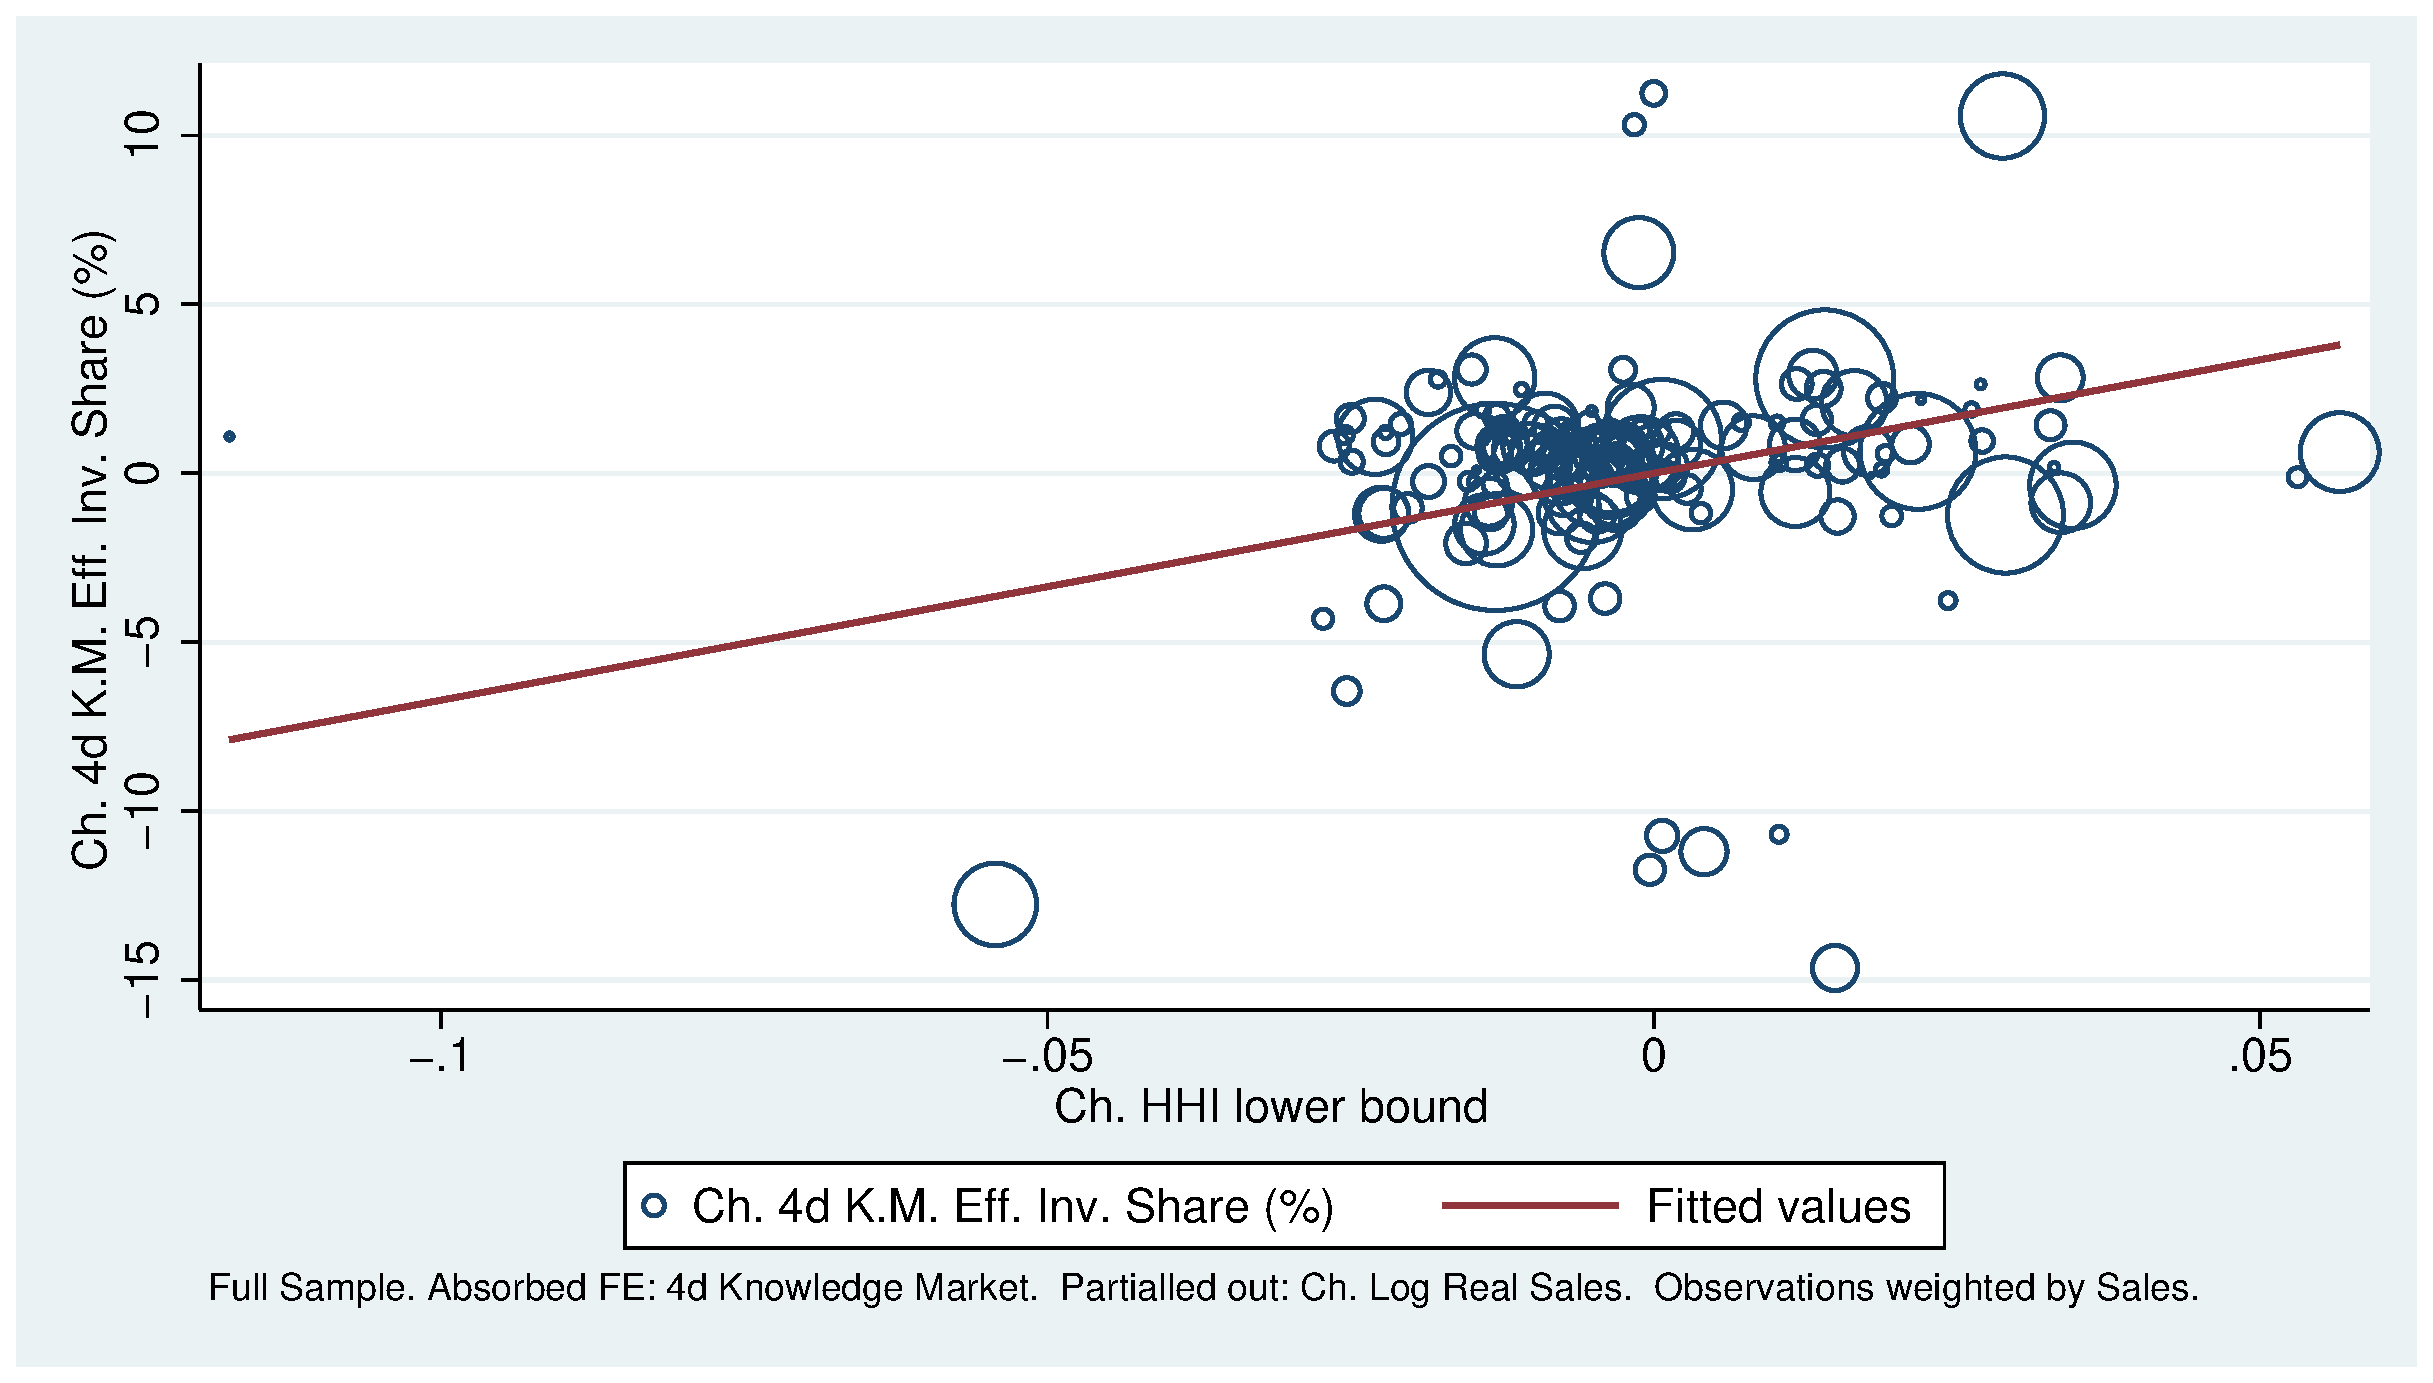
\includegraphics[width=0.9\textwidth]{../graphs/raw_Dk4_hhi_N_inv0}}

\subfloat[Binned Scatter Plot, Specification in Column (6)]{\centering{}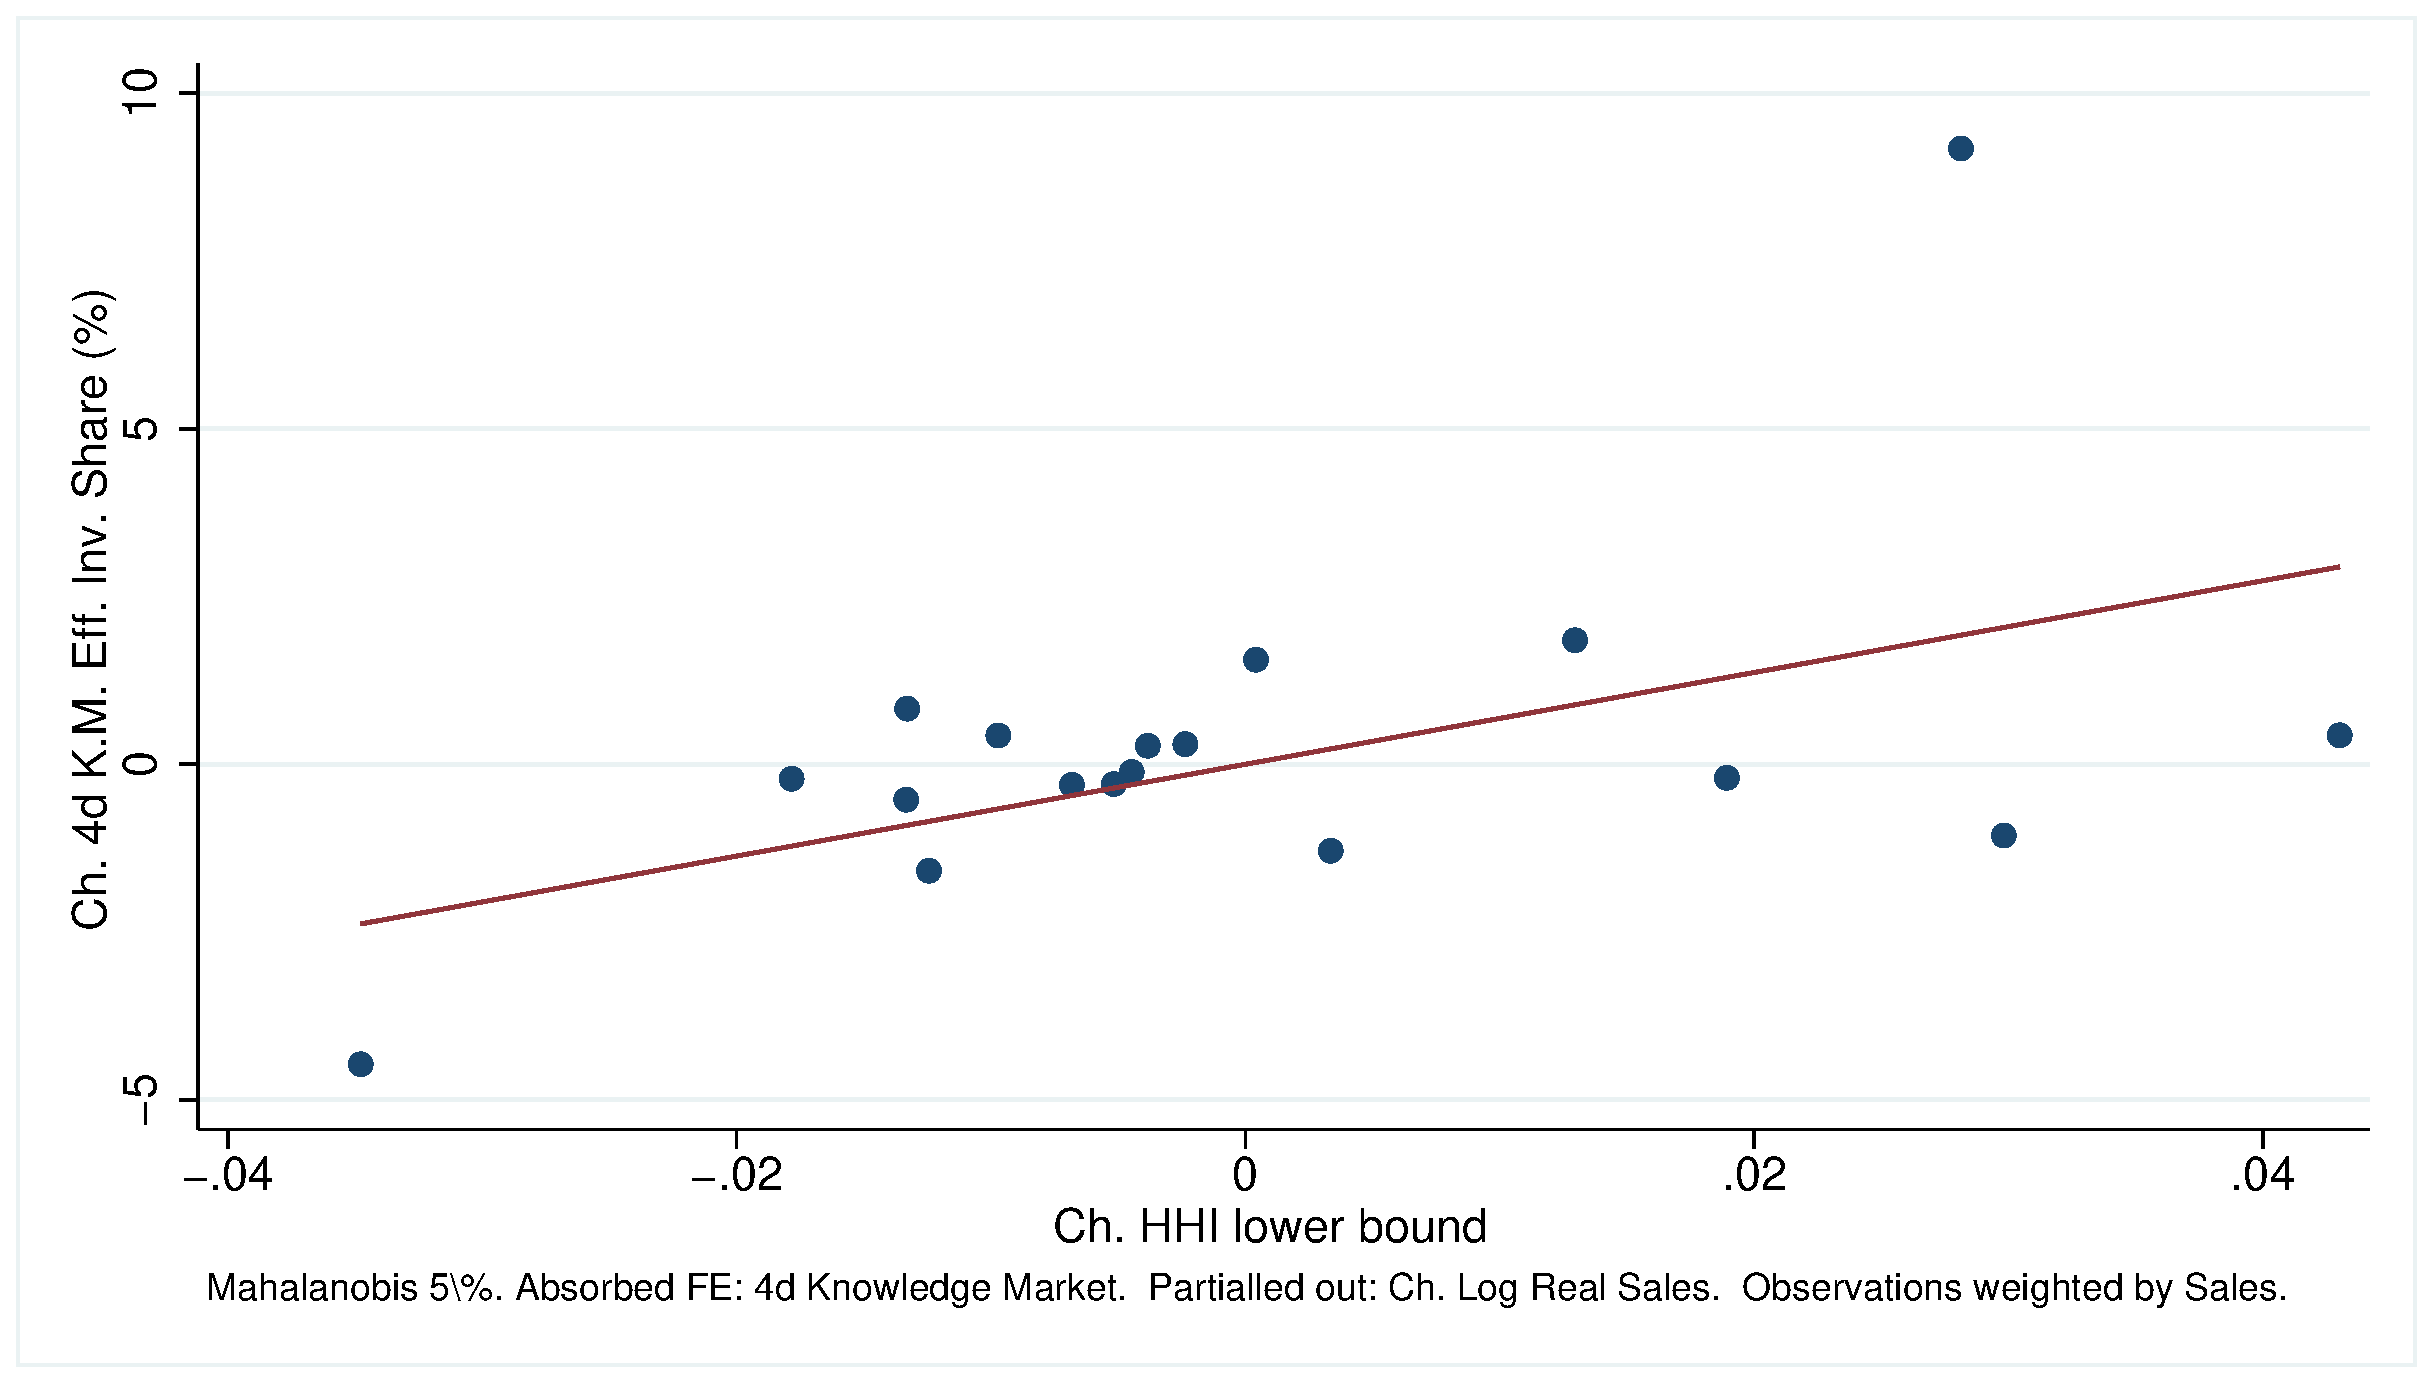
\includegraphics[width=0.9\textwidth]{../graphs/bin_Dk4_hhi_N_inv2}}\\

\raggedright{}{\small{}Note: This figure presents residualized scatter
plots of the change in the share of effective inventors of sector
$p$ over total inventors in knowledge market $k$, over the change
in the lower bound of the Herfindal-Hirschman Index for product market
$p$, as implied by Census concentration ratios. The upper panel reports
the data corresponding to the full sample, where both variables have
been residualized by change in log real sales and knowledge market
fixed effects. The size of the markers is proportional to the weight
of each observation in the regression, corresponding to total sector
sales in 2012. The regression line corresponds to the coefficient
on the change in HHI lower bound reported in Column (2) of Table }\ref{tab: RegShInvHHI-1}{\small{}.
The lower panel presents a binned scatter plot on the sample where
the observations with the highest 5\% Mahalanobis distance from sample
centroid have been removed. Observations are aggregated using sales
weights and the regression line results from the specification in
Column (6) of Table }\ref{tab: RegShInvHHI-1}{\small{}.}{\small\par}
\end{figure}
\FloatBarrier

\subsection{Using a Quartic in Sales as Size Control}

This Section displays the results of estimating the specification
in Table \ref{tab: RegShInvHHI} using the changes in the terms of
a fourth-degree polynomial in sales rather than log-sales. This flexible
control specification ensures that my main findings do not rely on
the specific functional form that I assumed above. Table \ref{tab: RegShInvQuartic}
reports the result of this exercise using both effective inventors
(Columns (1) and (2)) and raw inventor counts (Columns (3) and (4))
to compute sector shares. Recall that when using raw inventor counts,
knowledge markets are also constructed according to this measure.
As clear from a comparison of Columns (1) with (2), and (3) with (4),
these two specifications produce statistically undistinguishable results.

\begin{table}[th]
\caption{Regressions of Change in 4-digit Knowledge Market Share of Inventors
over Change in HHI Lower Bound, Long-Differences, 1997-2012\label{tab: RegShInvQuartic}}

\begin{centering}
\scalebox{.9}{{
\def\sym#1{\ifmmode^{#1}\else\(^{#1}\)\fi}
\begin{tabular}{l*{4}{c}}
\hline\hline
                    &$\Delta$ Inventor Share (pp)   &               &               &               \\
                    &\multicolumn{1}{c}{(1)}   &\multicolumn{1}{c}{(2)}   &\multicolumn{1}{c}{(3)}   &\multicolumn{1}{c}{(4)}   \\
\hline
$\Delta \underline{\text{HHI}}$&      22.509*  &      24.083*  &      67.160+  &      74.769+  \\
                    &    (10.848)   &    (10.565)   &    (37.176)   &    (39.225)   \\
$\Delta \log$ Sales &       0.548*  &               &       1.422*  &               \\
                    &     (0.243)   &               &     (0.717)   &               \\
$\Delta$ Sales ($\$$ bn)&               &       2.617*  &               &       6.382+  \\
                    &               &     (1.108)   &               &     (3.365)   \\
$\Delta \text{Sales}^2$ &               &      -0.749   &               &      -1.749   \\
                    &               &     (0.482)   &               &     (1.468)   \\
$\Delta \text{Sales}^3$ &               &       0.081   &               &       0.165   \\
                    &               &     (0.076)   &               &     (0.232)   \\
$\Delta \text{Sales}^4$ &               &      -0.003   &               &      -0.005   \\
                    &               &     (0.003)   &               &     (0.009)   \\
\hline
4D Knowledge Market FE&   \ding{51}   &   \ding{51}   &   \ding{51}   &   \ding{51}   \\
Sample              & Full Sample   & Full Sample   & Full Sample   & Full Sample   \\
Weight              &       Sales   &       Sales   &       Sales   &       Sales   \\
Observations        &         153   &         153   &         156   &         156   \\
\hline\hline
\end{tabular}
}
}
\par\end{centering}
\raggedright{}{\small{}Note: Regressions weighted by sales in 2012;
Robust standard errors in parentheses; Symbols denote significance
levels $\left(+\ p<0.1,^{*}\ p<0.05,^{**}\ p<.01,^{***}\ p<.001\right)$;
Checkmarks indicate the inclusion of fixed effects. This Tables presents
the results of specifications (\ref{eq: spec}), when the outcome
is the share of effective inventors of sector $p$ over total inventors
in knowledge market $k$, and the independent variable is the change
in the lower bound of the Herfindal-Hirschman Index for product market
$p$, as implied by Census concentration ratios. ``Full Sample''
refers to the sample described in the main text.}{\small\par}
\end{table}


\subsection{Using the HHI as the Independent Variable in Patent Quality Regressions\label{subsec:Patents-with-HHI}}

This Section reports the results analogous to Tables \ref{tab: RegStats}
and \ref{tab: RegFwdCite} in the main text, using the HHI lower bound
as the independent variable rather than the share of inventors. As
should be expected from the high correlation between the two variables,
the results are qualitatively similar to those reported there, with
some distinctions. First, Table \ref{tab: RegStats-1} confirms that
there has a been a large and significant increase in the concentration
of inventors among top firms in product market with increasing HHI.
Differently from the main specification, this seems to be driven primarily
by a fall in the share of the bottom half innovative firms. However,
this does not counter the interpretation provided in the main text
that increased concentration tends to reduce entry, which manifests
in these regressions through a fall in the share of inventors employed
by smaller, and presumably younger, firms. Table \ref{tab: RegFwdCite-1}
shows the robustness of my findings on forward citations to the use
of the HHI as well as weighting the regressions by 2012 sales, although
the generality coefficient appears non-significant, as discussed in
the main text.

\begin{sidewaystable}[ph]
\caption{Regressions of Change in Inventor Distribution Measures over Change
in 4-digit Knowledge Market Share, Long-Difference, 1997-2012\label{tab: RegStats-1}}

\begin{centering}
\scalebox{1}{{
\def\sym#1{\ifmmode^{#1}\else\(^{#1}\)\fi}
\begin{tabular}{l*{5}{c}}
\hline\hline
                    &Ch. Inv. 90/50 Quantile Ratio   &$\Delta$ Top 10\\%/Bottom 50\\%   &Ch. Inv. Top-50/Bottom-50 Share Ratio   &$\Delta$ Top 10\\%   &$\Delta$ Bottom 50\\%   \\
                    &\multicolumn{1}{c}{(1)}   &\multicolumn{1}{c}{(2)}   &\multicolumn{1}{c}{(3)}   &\multicolumn{1}{c}{(4)}   &\multicolumn{1}{c}{(5)}   \\
\hline
$\Delta \underline{\text{HHI}}$&      15.426*  &       1.793   &      10.566   &      -0.085   &      -0.409*  \\
                    &     (6.848)   &     (5.797)   &     (8.078)   &     (0.539)   &     (0.188)   \\
$\Delta \log$ Sales &       0.048   &       0.464   &       0.340   &       0.036   &      -0.000   \\
                    &     (0.154)   &     (0.349)   &     (0.407)   &     (0.022)   &     (0.008)   \\
\hline
Knowledge Market FE &   \ding{51}   &   \ding{51}   &   \ding{51}   &   \ding{51}   &   \ding{51}   \\
Sample              & Full Sample   & Full Sample   & Full Sample   & Full Sample   & Full Sample   \\
Weight              &       Sales   &       Sales   &       Sales   &       Sales   &       Sales   \\
Observations        &         118   &         118   &         118   &         118   &         118   \\
\hline\hline
\end{tabular}
}
}\\
\par\end{centering}
\raggedright{}{\small{}Note: Regressions weighted by sales in 2012;
Robust standard errors in parentheses; Symbols denote significance
levels $\left(+\ p<0.1,^{*}\ p<0.05,^{**}\ p<.01,^{***}\ p<.001\right)$;
Checkmarks indicate the inclusion of fixed effects. Please refer to
notes in Table \ref{tab: RegShInvHHI} for further details. Column
(1) uses the ratio in the 90 percentile of effective inventors to
the median as the outcome variable. Columns (2) and (3) instead present
the share ratio, that is the share of effective inventors accruing
to the top 10 or 50\% relative to the share accruing to the bottom
50\% of the distribution within each NAICS sector.}{\small\par}
\end{sidewaystable}

\begin{table}
\caption{Regressions of Changes in Forward Citation over HHI Changes, Long-Differences,
1997-2012\label{tab: RegFwdCite-1}}

\begin{centering}
\subfloat[Full sample]{\begin{centering}
\par\end{centering}
\centering{}\scalebox{.9}{{
\def\sym#1{\ifmmode^{#1}\else\(^{#1}\)\fi}
\begin{tabular}{l*{3}{c}}
\hline\hline
                    &$\Delta \log$ Citations/Patent (CPC)   &$\Delta \log$ Citations/Patent (Total)   &$\Delta$ Patent Generality   \\
                    &\multicolumn{1}{c}{(1)}   &\multicolumn{1}{c}{(2)}   &\multicolumn{1}{c}{(3)}   \\
\hline
$\Delta \underline{\text{HHI}}$&     -11.133** &     -12.524** &      -0.335   \\
                    &     (3.730)   &     (4.324)   &     (0.431)   \\
$\Delta \log$ Sales &      -0.454*  &      -0.523*  &      -0.019   \\
                    &     (0.201)   &     (0.257)   &     (0.022)   \\
\hline
Knowledge Market FE &   \ding{51}   &   \ding{51}   &   \ding{51}   \\
Sample              & Full Sample   & Full Sample   & Full Sample   \\
Weight              &       Sales   &       Sales   &       Sales   \\
Observations        &         153   &         153   &         153   \\
\hline\hline
\end{tabular}
}
}}
\par\end{centering}

\begin{centering}
\subfloat[Full sample, restricting to the middle range of the change in inventor
shares ($-2\%$ to $+2\%$)]{\centering{}\scalebox{.9}{ {
\def\sym#1{\ifmmode^{#1}\else\(^{#1}\)\fi}
\begin{tabular}{l*{3}{c}}
\hline\hline
                    &$\Delta \log$ Citations/Patent (CPC)   &$\Delta \log$ Citations/Patent (Total)   &$\Delta$ Patent Generality   \\
                    &\multicolumn{1}{c}{(1)}   &\multicolumn{1}{c}{(2)}   &\multicolumn{1}{c}{(3)}   \\
\hline
$\Delta \underline{\text{HHI}}$&     -10.646** &     -13.052** &      -0.624   \\
                    &     (4.018)   &     (4.979)   &     (0.473)   \\
$\Delta \log$ Sales &      -0.467*  &      -0.554*  &      -0.022   \\
                    &     (0.214)   &     (0.273)   &     (0.023)   \\
\hline
Knowledge Market FE &   \ding{51}   &   \ding{51}   &   \ding{51}   \\
Sample              & Full Sample   & Full Sample   & Full Sample   \\
Weight              &       Sales   &       Sales   &       Sales   \\
Observations        &         144   &         144   &         144   \\
\hline\hline
\end{tabular}
}
}}\\
\par\end{centering}
\raggedright{}{\small{}Note: Unweighted regressions; Robust standard
errors in parentheses; Symbols denote significance levels $\left(+\ p<0.1,^{*}\ p<0.05,^{**}\ p<.01,^{***}\ p<.001\right)$;
Checkmarks indicate the inclusion of fixed effects. This Tables presents
the results of specification (\ref{eq: specFE}), when the outcome
is the log-change in forward citations and the change in patent generality
in sector $p$ over the change in the share of inventors employed
in sector $p$. Column (1) and (2) presents the results when forward
citations are extrapolated the procedure Hall et al. (2000) to avoid
truncation bias. A specific cite-lag distribution over 35 years is
estimated for each pair of cited and citing CPC2-codes. Column (1)
employs the extrapolation scheme by each pair of CPC2 cited and citing
sector. Column (2) applies the extrapolation scheme to total citations
received by each cited patent. Column (3) presents results on the
patent generality measures. All columns exclude self-citations. Upper
panel: full sample; Bottom panel: excluding sectors with absolute
increase in the inventor share above 2\%.}{\small\par}
\end{table}


\subsection{Using the Lerner Index instead of the HHI\label{app:Using-the-Lerner}}

Following \citet{grullonAreUSIndustries2019a}, I build the Lerner
Index from NBER-CES data for the period 1997-2012 as the ratio:
\begin{equation}
\text{Lerner}_{jt}=\frac{\text{vship}_{jt}-\text{pay}_{jt}-\text{matcost}_{jt}-\text{energy}_{jt}}{\text{vship}_{jt}},\label{eq: Lerner}
\end{equation}
where ``vship'' is the total value of shipments, ``pay'' denotes
total payrolls, ``matcost'' and ``energy'' material and energy
costs, respectively, and $j$ denotes a 6- or 4-digit NAICS sector.
I build two alternative measures, one using 6-digit NAICS sectors,
the original identifier in NBER-CES, and then averaging by sales at
the level of 4-digit NAICS, or first aggregating the revenue and cost
statistics at the level of 4-digit NAICS. Table \ref{tab: LernerVHHI},
shows that the Lerner Index thus constructed is strongly correlated
with the HHI measure used in the main analysis. However, the correlation
is far from perfect, as suggested by the $R^{2}$, suggesting that
this estimate of the Lerner Index might be excessively imprecise.
Indeed, Table \ref{tab: MainWLerner} shows that, when using this
measure instead of the HHI in the main analysis, the coefficients
for the regression of inventors' shares on changes in concentration
stay positive, but become smaller and noisier. This suggests the potential
presence of attenuation bias, a valid concern due to the fact that
the above measure, not based on any structural estimation, can only
imperfectly capture markups. Note that this is also due to the fact
that the Lerner Index is available only for the manufacturing sectors,
which make up about 60\% of the sample, so its use lead to dropping
a substantial amount of observations. When using fitted values from
the regression in Table \ref{tab: LernerVHHI} to extend the measure
to more sectors, as well as reducing the volatility of the series
for available sectors, the coefficients recover magnitudes and significance
close to the baseline presented in \ref{tab: RegShInvHHI}.

\begin{table}[h]
\caption{Regressions of Changes in the Lerner Index over Changes in the HHI
Lower Bound, Long-Difference, 1997-2012\label{tab: LernerVHHI}}

\begin{centering}
\scalebox{1}{{
\def\sym#1{\ifmmode^{#1}\else\(^{#1}\)\fi}
\begin{tabular}{lHc}
\hline\hline
                    &Markup Change 1997-2012, 6d Lerner Index   & $\Delta$ Lerner Index   \\
                    &\multicolumn{1}{H}{(1)}   &\multicolumn{1}{c}{(2)}   \\
\hline
$\Delta \underline{HHI}$&       1.490***&       1.652***\\
                    &     (0.229)   &     (0.257)   \\
\hline
Observations        &         258   &         258   \\
R-squared           &    .1424476   &     .14   \\
\hline\hline
\end{tabular}
}
}\\
\par\end{centering}
\raggedright{}{\small{}Note: Robust standard errors in parentheses;
Symbols denote significance levels $\left(+\ p<0.1,^{*}\ p<0.05,^{**}\ p<.01,^{***}\ p<.001\right)$.
``6d Lerner Index'' refers to the Lerner Index constructed as in
(\ref{eq: Lerner})on NAICS 6-digits averaged at the 4-digit NAICS
level weighting by the value of shipments; ``4d Lerner Index'' is
computed using 4-digit aggregates for the value of shipments, payroll
and costs, summing over the NAICS 6-digit composing each sector. }{\small\par}
\end{table}

\begin{table}[h]
\caption{Regressions of Changes in Inventors' Share over Changes in Actual
and Fitted Lerner Index, Long-Difference, 1997-2012\label{tab: MainWLerner}}

\begin{centering}
{
\def\sym#1{\ifmmode^{#1}\else\(^{#1}\)\fi}
\begin{tabular}{l*{2}{c}}
\hline\hline
                    &Ch. 4d K.M. Eff. Inv. Share (\%)   &               \\
                    &\multicolumn{1}{c}{(1)}   &\multicolumn{1}{c}{(2)}   \\
\hline
Markup Change 1997-2012, 4d Lerner Index&       0.556   &               \\
                    &     (5.465)   &               \\
Fitted Lerner Change&               &      26.736*  \\
                    &               &    (13.363)   \\
\hline
4D Knowledge Market &               &               \\
Sample              & Full Sample   & Full Sample   \\
Weight              &       Sales   &       Sales   \\
Observations        &          81   &         157   \\
\hline\hline
\end{tabular}
}
\\
\par\end{centering}
\raggedright{}{\small{}Note: Robust standard errors in parentheses;
Symbols denote significance levels $\left(+\ p<0.1,^{*}\ p<0.05,^{**}\ p<.01,^{***}\ p<.001\right)$;
Observations weighted by sales. The markup change 1997-2012 is the
long-difference of the Lerner Index described above. ``Fitted Lerner
change'' is the fitted value for the Lerner index based on the estimates
in \ref{tab: LernerVHHI}, and extended to all available sectors in
the main sample. }{\small\par}
\end{table}
\FloatBarrier

\section{Omitted Proofs and Derivations\label{app: Omitted-Proofs}}

\subsection{One-sector model}

\begin{proof}[Proof of Proposition \ref{prop: partialEq}]
 This proof consists of several parts. First, I show that given labor
supplies, output, values and wages grow at the same constant rate,
so the problem can be solved in a steady state of a normalized model.
Second, show that normalized values, $v(\Omega)\equiv V_{t}(\Omega)/Y_{t}$,
are uniquely determined, which gives unique research intensities and
stationary distribution. Third, I derive the stationary distribution
and the expression for growth and inventors' productivity. In what
follows I suppress stars to denote equilibrium quantities for ease
of notation.

Given an endowment, $L$, production labor market clearing in each
period requires:
\[
\int_{0}^{1}l_{i,t}(w)d(i)=L.
\]
That is,
\[
L=\int_{0}^{1}\frac{c_{i,t}}{\phi}y_{i,t}\left(w_{t}\right)d(i)=\frac{1}{\phi}\frac{Y_{t}}{w_{t}},
\]
where the second equality comes from using the demand for output of
product $i$ for $y_{i,t}\left(w_{t}\right)$. This expression immediately
implies that if $Y_{t}$ grows at a constant rate, so does $w_{t}$.
Labor market clearing for R\&D workers reads:
\[
L^{RD}=\zeta\omega x_{e,\omega}\left(\mu_{e,\omega}+\mu_{e,1}\right)+\alpha_{I}\frac{\left(x_{I}\right)^{\gamma}}{\gamma}\mu_{1}.
\]
 In a constant growth equilibrium (CGE), the distribution is stationary,
and since the left hand side is constant, research intensities are
also fixed. A contradiction arises otherwise, since the distribution
is stationary only if research intensities are fixed by the LOM (\ref{eq: StatDist1})-(\ref{eq: statDist4}).
Further, R\&D labor cannot grow since the growth rate in the economy
increases in total R\&D labor for any given distribution, as it will
be clear below. The fact that research intensities are constant immediately
implies, from the optimality of $x_{e,\omega}$, that $V_{t}(1)$
and $w_{t}^{RD}$ grow at the same rate. Indeed, from the FOC for
entrants' research:
\[
0=\mathrm{d}\log x_{e,\omega,t}=\mathrm{d}\log V_{t}(1)-\mathrm{d}\log w_{t}^{RD}.
\]
This result in turn implies, combined with the FOC for $x_{I},$ that
$V_{t}(\omega)$ also grows at the same constant rate. Now consider
the budget constraint of the representative household, combined with
product market clearing, $Y_{t}=C_{t}$: 
\[
r_{t}A_{t}-\dot{A}_{t}+w_{t}^{RD}L^{RD}+w_{t}L=Y_{t},
\]
where $A_{t}$ denote the household's assets, that is all firms in
the economy. Therefore the above reads:
\[
r_{t}\left(\mu_{1}V_{t}(1)+\mu_{\omega}V_{t}(\omega)\right)-\mu_{1}\dot{V}_{t}(1)-\mu_{\omega}\dot{V}_{t}(\omega)+w_{t}^{RD}L^{RD}+w_{t}L=Y_{t}
\]
Dividing both sides by $V(1)$, using the Euler equation and rearranging
we obtain:
\[
\left(g+\rho\right)\left(\mu_{1}+\mu_{\omega}\frac{V_{t}(\omega)}{V_{t}(1)}\right)-\mu_{1}g_{V_{1}}-\mu_{\omega}\frac{V_{t}(\omega)}{V_{t}(1)}g_{V_{1}}+\frac{w_{t}^{RD}}{V_{t}(1)}L^{RD}=\frac{Y_{t}}{V_{t}(1)}-\frac{w_{t}}{V_{t}(1)}L.
\]
By what shown above, all terms on the left hand side are constant
in $t$, since research wages and values grows at the same rate and
the distribution is stationary. Since $Y_{t}$ and $w_{t}$ grow at
the same rate positive rate, it must be that $V_{t}(1)$ also grows
at the same rate as $Y_{t}$. This proves that $g_{V_{1}}=g=g_{c}=g_{w}=g_{w^{RD}}.$

As a result, in a CGE, it is possible to define normalized constant
values, $v(\Omega)\equiv V_{t}(\Omega)/Y_{t}$. The system of equations
defining the recursive problem in this equilibrium reads:
\begin{align}
\rho v(1) & =\max_{x_{I}}\left\{ \left(\frac{\phi-1}{\phi}\right)-\alpha_{I}\frac{x_{I}^{\gamma}}{\gamma}w^{RD}+x_{I}\left(v(\omega)-v(1)\right)-x_{e,1}v(1)\right\} ,\label{eq:normV1}\\
\rho v(\omega) & =\left(\frac{\phi-1}{\phi}\right)+\delta\left(v(1)-v(\omega)\right)-x_{e,\omega}v(\omega),\label{eq:normVom}
\end{align}
where the left hand side comes from using the Euler equation:
\[
r=g+\rho
\]
Which gives 
\[
r\frac{V_{t}(\Omega)}{Y_{t}}-\frac{\dot{V}_{t}(\Omega)}{Y_{t}}\frac{Y_{t}}{\dot{Y}_{t}}\frac{\dot{Y_{t}}}{V_{t}(\Omega)}\frac{V_{t}(\Omega)}{Y_{t}}=\left(\rho+g\right)v(\Omega)-gv(\Omega)=\rho v(\Omega).
\]

I now move to show that normalized values (\ref{eq:normV1}) and (\ref{eq:normVom})
are uniquely determined. Given entrants' decisions, and a wage rate
$w^{RD},$ the incumbent's choice of R\&D satisfies:
\[
x_{I}=\bm{1}\left\{ v(\omega)-v(1)>0\right\} \left(\frac{v(\omega)-v(1)}{\alpha_{I}w^{RD}}\right)^{\frac{1}{\gamma-1}}.
\]
Entrants taking $x_{I}$ as given optimally set:
\[
x_{e,1}=\bm{1}\left\{ v(1)>0\right\} \frac{v(1)}{\zeta w^{RD}},\quad x_{e,\omega}=\bm{1}\left\{ v(1)>0\right\} \frac{v(1)}{\zeta\omega w^{RD}}.
\]
Note that these solutions immediately imply that the normalized value,
$v(1)$, is strictly positive. Indeed, $v(1)<0$ would imply:
\[
\rho v(1)=\pi+\bm{1}\left\{ v(\omega)-v(1)>0\right\} \left(\frac{\gamma-1}{\gamma}\left(\frac{v(\omega)-v(1)}{\alpha_{I}w^{RD}}\right)^{\frac{1}{\gamma-1}}\right)\left(v(\omega)-v(1)\right)
\]
where the right hand side is strictly positive. Plugging optimal solutions
into the system of equations determining the value functions (\ref{eq: normV1})
and (\ref{eq: normV2}) gives:
\begin{align}
\rho v(1)-\pi-\bm{1}\left\{ v(\omega)-v(1)>0\right\} \left(\frac{\gamma-1}{\gamma}\left(\frac{v(\omega)-v(1)}{\alpha_{I}w^{RD}}\right)^{\frac{1}{\gamma-1}}\right)\left(v(\omega)-v(1)\right)+\frac{v(1)^{2}}{\zeta w^{RD}} & =0\label{eq: sys1-3}\\
\rho v(\omega)-\pi-\delta\left(v(1)-v(\omega)\right)+\frac{v(1)}{\zeta w^{RD}\omega}v(\omega) & =0.\label{eq: sys2-3}
\end{align}
The second equation gives $v(\omega)$ as the following function of
$v(1):$
\[
v(\omega)=\frac{\pi+\delta v(1)}{\rho+\delta+\frac{v(1)}{\zeta w^{RD}\omega}}.
\]

Suppose first that $v(\omega)<v(1).$ In this case, the first equation
gives:
\[
\rho v(1)+\frac{v(1)^{2}}{\zeta w^{RD}}-\pi=0.
\]
The roots of this equation are:
\[
v_{1,2}=\frac{-\rho\pm\sqrt{\rho^{2}+4\frac{\pi}{\zeta w^{RD}}}}{\frac{2}{\zeta w^{RD}}}.
\]
Since the term under the root is strictly positive, only one of these
roots is admissible, so the above system is solved for a unique pair
$v(1),v(\omega).$ Consider now the case $v(\omega)>v(1).$ It is
straightforward to note that $v(\omega)-v(1)$ is decreasing in $v(1).$
This implies that, when rewriting (\ref{eq: sys1-3}) as
\begin{equation}
-\left(\frac{\gamma-1}{\gamma}\left(\frac{v(\omega)-v(1)}{\alpha_{I}w^{RD}}\right)^{\frac{1}{\gamma-1}}\right)\left(v(\omega)-v(1)\right)=\pi-\rho v(1)-\frac{v^{2}(1)}{\zeta w^{RD}},\label{eq:solV1}
\end{equation}
the left hand side is monotonically increasing in $v(1)$, while the
right hand side is monotonically decreasing in $v(1)$. Further, at
$v(1)=0$, the left hand side is strictly negative, while the right
hand side equals $\pi$, while for $v(1)\rightarrow\infty$, the right
hand side tends to $+\infty$ while the left hand side decreases towards
$-\infty$. As a result, (\ref{eq:solV1}) has a unique positive solution. 

The uniqueness of $v(1)$ immediately implies unique $v(\omega)$
and R\&D choices. Given these R\&D choices, the stationary distribution
satisfies 
\begin{align}
0 & =-\left(x_{I}+x_{e,1}\right)\mu_{1}+\delta\mu_{\omega}+x_{e,\omega}\mu_{e,\omega}+x_{e,1}\mu_{e,1},\label{eq: dist1-2}\\
0 & =-\left(x_{e,\omega}+\delta\right)\mu_{\omega}+x_{I}\mu_{1},\label{eq: dist2-2}\\
0 & =-\left(x_{e,1}+x_{I}\right)\mu_{e,1}+x_{e,1}\mu_{1}+\delta\mu_{e,\omega},\label{eq: dist3-3}\\
0 & =-\left(x_{e,\omega}+\delta\right)\mu_{e,\omega}+x_{e,\omega}\mu_{\omega}+x_{I}\mu_{e,1}.\label{eq: dist4-3}
\end{align}
By equation (\ref{eq: dist2-2}):
\[
x_{I}\mu_{1}=\left(x_{e,\omega}+\delta\right)\mu_{\omega}
\]
Since $\mu_{1}=1-\mu_{\omega}$, the stationary distribution has:
\begin{align}
\mu_{\omega} & =\frac{x_{I}}{x_{I}+x_{e,\omega}+\delta},\nonumber \\
\mu_{1} & =\frac{x_{e,\omega}+\delta}{x_{I}+x_{e,\omega}+\delta},\nonumber \\
\left[\begin{matrix}-\delta & x_{e,1}+x_{I}\\
x_{e,\omega}+\delta & -x_{I}
\end{matrix}\right] & \left[\begin{matrix}\mu_{e,\omega}\\
\mu_{e,1}
\end{matrix}\right]=\left[\begin{matrix}x_{e,1}\mu_{1}\\
x_{e,\omega}\mu_{\omega}
\end{matrix}\right].\label{eq:sys}
\end{align}
Since the matrix in (\ref{eq:sys}) is nonsingular, $\mu_{e,\omega}$
and $\mu_{e,1}$ are uniquely determined as: 
\begin{align*}
\mu_{e,\omega} & =\frac{x_{I}x_{e,1}\mu_{1}+\left(x_{e,1}+x_{I}\right)x_{e,\omega}\mu_{\omega}}{x_{e,\omega}\left(x_{e,1}+x_{I}\right)+\delta x_{e,1}},\\
\mu_{e,1} & =\frac{\left(x_{e,\omega}+\delta\right)x_{e,1}\mu_{1}+\delta x_{e,\omega}\mu_{\omega}}{x_{e,1}\left(x_{e,\omega}+\delta\right)+x_{e,\omega}x_{I}}
\end{align*}
By the optimal solution for entrants:
\[
x_{e,1}=\omega x_{e,\omega},
\]
so (\ref{eq:sys}) is solved for:
\begin{align}
\mu_{e,\omega} & =\frac{\omega x_{I}\mu_{1}+\left(\omega x_{e,\omega}+x_{I}\right)\mu_{\omega}}{\omega\left(x_{e,\omega}+\delta\right)+x_{I}},\label{eq: mu_e_om}\\
\mu_{e,1} & =\frac{\omega\left(x_{e,\omega}+\delta\right)\mu_{1}+\delta\mu_{\omega}}{\omega\left(x_{e,\omega}+\delta\right)+x_{I}}.\label{eq: mu_e_1}
\end{align}
Thus, the stationary distribution is unique. 

It remains to show that equilibrium R\&D labor is also unique. To
show this, I prove that R\&D labor demand is monotonically decreasing
in wages and has:
\[
\lim_{w^{RD}\rightarrow\infty}L^{RD}(w^{RD})\leq0,\quad\lim_{w^{RD}\rightarrow0}L^{RD}(w^{RD})=\infty.
\]
 Since the converse holds for R\&D labor supply is monotonically increasing
in wages and ranges between $0$ and $+\infty$, this gives a unique
intersection of the two schedules. First note that, if labor supply
is inelastic, $\phi=0,$ equilibrium R\&D labor is constant by definition.
Lemma \ref{lem:Labor Demand} below builds on this observation as
well as \ref{lem: values} to prove that research labor demand is
indeed monotonically decreasing in the wage.
\begin{lem}
\label{lem: values}Consider a steady state of the normalized one-sector
model, and assume that defensive innovation is effective, $\omega>1$.
Then, $\omega v(1)>v(\omega)>v(1).$ Around a steady state, and for
a fixed wage rate, $w^{RD}$, the normalized values, $v(1),v(\omega)$,
are increasing in the markup, $\phi$, and
\[
\frac{\partial v(\omega)}{\partial\phi}>\frac{\partial v(1)}{\partial\phi}>0.
\]
\end{lem}
%
\begin{proof}[Proof of Lemma \ref{lem: values}]
Subtracting side by side Equation (\ref{eq: sys1-3}) from (\ref{eq: sys2-3})
gives:
\begin{align*}
\left(\rho+\delta+\bm{1}\left\{ v(\omega)-v(1)>0\right\} \left(\frac{\gamma-1}{\gamma}\left(\frac{v(\omega)-v(1)}{\alpha_{I}w^{RD}}\right)^{\frac{1}{\gamma-1}}\right)\right)\left(v(\omega)-v(1)\right) & =\frac{v(1)}{\zeta w^{RD}}\left(v(1)-\frac{v(\omega)}{\omega}\right)
\end{align*}
Suppose that $v(\omega)<v(1)$. This implies that the left hand side
of the above expression is strictly smaller than $0$, while $\omega v(1)>v(1)>v(\omega),$
so the right hand side is strictly positive under the assumption $\omega>1$.
Therefore, it must be that $v(\omega)>v(1)$. If this is the case,
the left hand side is strictly positive, and to avoid a contradiction
it must be $\omega v(1)>v(\omega).$ Thus, $\omega v(1)>v(\omega)>v(1)$,
proving the first part of the statement.

Since $\pi$ is a monotone increasing function of $\phi$, I prove
the statement for value derivatives with respect to $\pi$. Total
differentiation of the system of Equations (\ref{eq: sys1-3}) and
(\ref{eq: sys2-3}) with respect to $\pi$ around a CGE gives
\begin{equation}
\underset{\equiv J}{\underbrace{\left[\begin{matrix}\rho+\left(\frac{v(\omega)-v(1)}{\alpha_{I}w^{RD}}\right)^{\frac{1}{\gamma-1}}+2\frac{v(1)}{\zeta} & -\left(\frac{v(\omega)-v(1)}{\alpha_{I}w^{RD}}\right)^{\frac{1}{\gamma-1}}\\
-\delta+\frac{v(\omega)}{\zeta w^{RD}\omega} & \rho+\delta+\frac{v(1)}{\zeta w^{RD}\omega}
\end{matrix}\right]}}\left[\begin{matrix}\mathrm{d}v(1)\\
\mathrm{d}v(\omega)
\end{matrix}\right]-\left[\begin{matrix}1\\
1
\end{matrix}\right]\mathrm{d}\pi=0.\label{eq: jacob}
\end{equation}
The determinant of the Jacobian is:
\begin{align*}
\det J & =\left(\rho+x_{I}+2\omega x_{e,\omega}\right)\left(\rho+\delta+\frac{v(1)}{\zeta\omega}\right)+x_{I}\left(x_{e,\omega}-\delta\right)>0.
\end{align*}
 Solving (\ref{eq: jacob}) gives:
\[
\left[\begin{matrix}\frac{\mathrm{d}v(1)}{\mathrm{d}\pi}\\
\frac{\mathrm{d}v(\omega)}{\mathrm{d}\pi}
\end{matrix}\right]=\frac{1}{\det J}\left[\begin{matrix}\frac{v(1)}{\zeta w^{RD}\omega}+\rho+\delta & \left(\frac{v(\omega)-v(1)}{\alpha_{I}w^{RD}}\right)^{\frac{1}{\gamma-1}}\\
\delta-\frac{v(\omega)}{\zeta w^{RD}\omega} & \rho+\left(\frac{v(\omega)-v(1)}{\alpha_{I}w^{RD}}\right)^{\frac{1}{\gamma-1}}+2\frac{v(1)}{\zeta w^{RD}}
\end{matrix}\right]\left[\begin{matrix}1\\
1
\end{matrix}\right].
\]
Since the first row is strictly positive, 
\[
\frac{\mathrm{d}v(1)}{\mathrm{d}\pi}>0.
\]
Subtracting line by line gives:
\begin{align}
\frac{\mathrm{d}v(\omega)}{\mathrm{d}\pi}-\frac{\mathrm{d}v(1)}{\mathrm{d}\pi} & =\frac{1}{\det J}\left[-\frac{v(\omega)}{\zeta w^{RD}\omega}-\rho+\frac{v(1)}{\zeta w^{RD}\omega}+\rho+2\frac{v(1)}{\zeta w^{RD}}\right]\nonumber \\
 & =\frac{1}{\det J}\left[-\frac{v(\omega)}{\zeta w^{RD}\omega}-\frac{v(1)}{\zeta w^{RD}\omega}+2\frac{v(1)}{\zeta w^{RD}}\right]\nonumber \\
 & =\frac{1}{\det J}\left[\frac{2\omega v(1)-\left(v(\omega)+v(1)\right)}{\zeta w^{RD}\omega}\right]>0\label{eq:diffVal}
\end{align}
since $\omega>1$ and $\omega v(1)>v(\omega),$ from what shown above.
It follows that: 
\[
\frac{\mathrm{d}v(\omega)}{\mathrm{d}\pi}>\frac{\mathrm{d}v(1)}{\mathrm{d}\pi}>0.
\]
 

\end{proof}
\begin{lem}
\label{lem:Labor Demand}R\&D labor demand is monotonically decreasing
in the wage rate $w_{t}^{RD}/Y_{t},$and:
\[
\lim_{w^{RD}\rightarrow\infty}L^{RD}(w^{RD})\leq0,\quad\lim_{w^{RD}\rightarrow0}L^{RD}(w^{RD})=\infty.
\]
\end{lem}
\begin{proof}
Consider the equilibrium with inelastic R\&D labor. By the resource
constraint in the economy, it holds:
\begin{align*}
\rho\left(\mu_{1}v(1)+\mu_{\omega}v(\omega)\right)+w^{RD}L^{RD}+wL & =1,\\
L^{RD} & =\frac{\pi}{w^{RD}}-\rho\left(\mu_{1}\frac{v(1)}{w^{RD}}+\mu_{\omega}\frac{v(\omega)}{w^{RD}}\right).
\end{align*}
Since the labor supply is fixed, shifts in the right hand side of
this equation identify the elasticity of labor supply to various parameters.
Now consider an increase in $\pi$ to $\pi'>\pi$. In this case, the
unique equilibrium requires:
\[
\frac{\pi'}{w^{RD\prime}}=\frac{\pi}{w^{RD}}.
\]
Indeed, guess that the equilibrium involves no changes in research
intensities, and therefore in the stationary distribution. Then:
\[
x'_{e,\omega}=x_{e,\omega}\Rightarrow\frac{v'(1)}{\zeta\omega w'^{RD}}=\frac{v(1)}{\zeta\omega w{}^{RD}},
\]
and
\[
x'_{I}=\left(\frac{v'(1)-v'(\omega)}{\alpha_{I}w'^{RD}}\right)^{\frac{1}{\gamma-1}}=\left(\frac{v(1)-v(\omega)}{\alpha_{I}w{}^{RD}}\right)^{\frac{1}{1-\gamma}}=x_{I}.
\]
As a result:
\[
\frac{v'(\omega)}{w'^{RD}}=\frac{v(\omega)}{w^{RD}}.
\]
Using the expression for $v(\omega),$ and using the fact that the
ratio between values and wages is the same in both equilibria, gives:
\[
\frac{\pi'}{w^{\prime RD}}=\frac{\pi}{w^{RD}}.
\]
This also ensures that:
\[
\rho\frac{v(1)}{w^{RD}}=\rho\frac{v'(1)}{w'^{RD}},
\]
 as is easily verified plugging the above expression into (\ref{eq:normV1})
evaluated at $\left(v(1),w^{RD}\right)$ and $\left(v'(1),w^{RD\prime}\right).$It
remains to show that goods' market clearing holds. Before a markup
change we have (in normalized values):
\begin{align*}
\rho\left(\mu_{1}v(1)+\mu_{\omega}v(\omega)\right)+w^{RD}L^{RD}+wL & =1,\\
\rho\left(\mu_{1}\frac{v(1)}{w^{RD}}+\mu_{\omega}\frac{v(\omega)}{w^{RD}}\right)+L^{RD} & =\frac{1-wL}{w^{RD}},
\end{align*}
By what shown above, with an inelastic labor research labor supply,
the left hand side has the same value before and after the change
in instantaneous profits. Further, the linear production function
implies that:
\[
wL=\frac{1}{\phi},
\]
therefore the right hand side can be written as:
\[
\frac{\pi}{w^{RD}},
\]
which has the same value in the new equilibrium. Therefore, the unique
equilibrium with inelastic labor supply is characterized by a constant
ratio $\frac{\pi}{w^{RD}}$. Given that the labor supply is inelastic,
$L^{RD}$ in the above expression can be read as the labor demand
for R\&D:\footnote{Alternatively, the market clearing expression can be rewritten as
the accounting identity that instantaneous profits equal the R\&D
wage bill plus dividends, which gives the demand for R\&D labor as
the expression reported below.}
\[
L^{RD,d}\left(w^{RD}\right)=\frac{\pi}{w^{RD}}-\rho\left(\mu_{1}\frac{v(1)}{w^{RD}}+\mu_{\omega}\frac{v(\omega)}{w^{RD}}\right)
\]
Now consider an initial equilibrium with $L^{RD,d}(w^{RD})=L^{d}$.
A change in the wage $w^{RD}$ to $w^{RD\prime}>w^{RD}$ modifies
the above expression to:
\[
L^{RD,d}\left(w^{RD\prime}\right)=\frac{\pi}{w^{RD\prime}}-\rho\left(\mu'_{1}\frac{v'(1)}{w^{RD\prime}}+\mu'_{\omega}\frac{v'(\omega)}{w^{RD\prime}}\right).
\]
By what shown above, it must be:
\[
\frac{\mathrm{d}\pi}{\pi}=\frac{w^{RD\prime}-w^{RD}}{w^{RD}}>0
\]
for $L^{RD,d}$ to be unchanged. Thus, denoting:
\[
\pi'=\pi\left(1+\frac{w^{RD\prime}-w^{RD}}{w^{RD}}\right),
\]
the above expression reads:
\[
L^{RD,d}\left(w^{RD\prime}\right)=\frac{\pi'}{w^{RD\prime}}+\frac{\pi-\pi'}{w^{RD\prime}}-\rho\left(\mu'_{1}\frac{v'(1)}{w^{RD\prime}}+\mu'_{\omega}\frac{v'(\omega)}{w^{RD\prime}}\right).
\]
That is:
\[
L^{RD,d}\left(w^{RD\prime}\right)=L^{RD,d}\left(w^{RD}\right)+\frac{\pi-\pi'}{w^{RD\prime}}<L^{RD,d}\left(w^{RD}\right).
\]
This shows that labor demand is decreasing in the wage. In general,
we have:
\[
L^{RD,d}\left(w^{RD\prime}\right)=L^{RD,d}\left(w^{RD}\right)+\frac{1}{w^{RD}}\left(\frac{w^{RD}}{w^{RD\prime}}-1\right)
\]
Consider now $w^{RD\prime}\rightarrow0,$ in this case we clearly
have:
\[
L^{RD,d}\left(w^{RD\prime}\right)\rightarrow\infty.
\]
Conversely, with $w^{RD\prime}\rightarrow\infty$: 
\[
L^{RD,d}\left(w^{RD\prime}\right)\rightarrow L^{RD,d}\left(w^{RD}\right)-\frac{1}{w^{RD}}=-\rho\left(\mu_{1}\frac{v(1)}{w^{RD}}+\mu_{\omega}\frac{v(\omega)}{w^{RD}}\right)-\frac{wL}{w^{RD}}<0.
\]
\end{proof}
By Lemma \ref{lem:Labor Demand}, given an endowment of production
labor and an R\&D labor supply schedule, the CGE is unique. 

To derive the growth rate note that, by the Cobb Douglas assumption
on the final good, and given the equilibrium wage rate for production
workers, $w=\frac{w_{t}}{Y_{t}},$
\begin{align*}
\log Y_{t} & =\int_{0}^{1}\log y_{t}(i)\mathrm{d}i\\
 & =\int_{0}^{1}\log\left(\frac{Y_{t}}{w_{t}c_{t}(i)}\right)\mathrm{d}i\\
 & =\int_{0}^{1}\log\left(\frac{1}{wc_{t}(i)}\right)\mathrm{d}i.
\end{align*}
It follows that:
\begin{align*}
g=\log\left(Y_{t+\Delta t}\right)-\log\left(Y_{t}\right) & =-\int_{0}^{1}\left(\log c_{t+\Delta}(i)-c_{t}(i)\right)\mathrm{d}i\\
 & =\eta\left[x_{e,\omega}\mu_{e,\omega}+x_{e,1}\mu_{e,1}+\lambda x_{I}\mu_{1}\right]\\
 & =\eta\left[x_{e,\omega}\left(\mu_{e,\omega}+\omega\mu_{e,1}\right)+\lambda x_{I}\mu_{1}\right].
\end{align*}
Productivity $g/L^{RD}$ follows directly from total R\&D labor demand:
\[
\zeta\omega x_{e,\omega}\left(\mu_{e,\omega}+\mu_{e,1}\right)+\alpha_{I}\frac{\left(x_{I}\right)^{\gamma}}{\gamma}\mu_{1}.
\]
\end{proof}
%
\begin{proof}[Proof of Proposition \ref{prop: partialEq}.]
 The increase in R\&D efforts by both incumbents and entrants descend
directly from Lemma \ref{lem: values}. In what follows, I derive
\emph{equilibrium }quantities, that is factoring in wage effects,
but I drop stars for ease of notation. 

To prove that the share of R\&D labor accruing to incumbents increases,
note first:
\[
\frac{\partial L_{I}}{\partial\phi}=\alpha_{I}x_{I}^{\gamma-1}\mu_{1}\frac{\partial x_{I}}{\partial\phi}+\frac{\alpha_{I}}{\gamma}x_{I}^{\gamma-1}\frac{\partial\left(x_{I}\mu_{1}\right)}{\partial\phi},
\]
where the first term is strictly positive, since I have prover that
$\frac{\partial x_{I}}{\partial\phi}>0,$ and the term, $\frac{\partial\left(x_{I}\mu_{1}\right)}{\partial\phi},$denotes
the derivative of aggregate incumbents' research intensity with respect
to the markup, and is also strictly positive. Indeed:
\begin{equation}
\frac{\partial\mu_{1}}{\partial\phi}=\frac{\partial\left(\frac{x_{e,\omega}+\delta}{x_{e,\omega}+\delta+x_{I}}\right)}{\partial\phi}=\left[\frac{\frac{\partial\left(x_{e,\omega}+\delta\right)}{\partial\phi}x_{I}-\left(x_{e,\omega}+\delta\right)\frac{\partial x_{I}}{\partial\phi}}{\left(x_{I}+x_{e,\omega}+\delta\right)^{2}}\right]=\mu_{1}\frac{\partial x_{I}}{\partial\phi}\frac{\left(\epsilon-1\right)}{\left(x_{I}+x_{e,\omega}+\delta\right)},\label{eq: der_Mu1}
\end{equation}
where I define the ratio of the elasticity of $x_{e,\omega}+\delta$
and $x_{I}$ to $\phi$ as:
\[
\epsilon\equiv\frac{\epsilon_{e}}{\epsilon_{I}}\equiv\frac{\nicefrac{\frac{\partial\left(x_{e,\omega}+\delta\right)}{\partial\phi}}{x_{e,\omega}}}{\nicefrac{\frac{\partial x_{I}}{\partial\phi}}{x_{I}}}\in(0,1].
\]
therefore:
\begin{align*}
\frac{\partial\left(\mu_{1}x_{I}\right)}{\partial\phi} & =\mu_{1}\frac{\partial x_{I}}{\partial\phi}\left[\frac{x_{I}\left(\epsilon-1\right)}{\left(x_{I}+x_{e,\omega}+\delta\right)}+1\right]\\
 & =\mu_{1}\frac{\partial x_{I}}{\partial\phi}\left[\frac{x_{I}\epsilon+x_{e,\omega}+\delta}{\left(x_{I}+x_{e,\omega}+\delta\right)}\right]>0.
\end{align*}
This proves that the aggregate incumbents' research intensity, $x_{I}\mu_{1}$,
is increasing in the markup. By (\ref{eq: der_Mu1}), $\mu_{1}$ decreases
with $\phi$ if and only if $\epsilon<1$, that is, $x_{I}$ is more
elastic than $x_{e,\omega}$ to changes in the markup. Therefore,
I now proceed to show that, when $\lambda=0,$ productivity is unambiguously
decreasing in $\phi$ if the mass of unprotected markets, $\mu_{1}$,
falls with $\phi$. With $\lambda=0$, inventors' productivity reads:
\begin{align*}
\frac{g}{L^{RD}} & =\eta\frac{x_{e,\omega}\left(\mu_{e,\omega}+\omega\mu_{e,1}\right)}{L_{e}+L_{I}},\\
 & =\eta\frac{x_{e,\omega}\left(\mu_{e,\omega}+\omega\mu_{e,1}\right)}{L_{e}\left(1+\frac{L_{I}}{L_{e}}\right)}\\
 & =\frac{\eta}{\zeta\omega}\underset{\equiv R}{\underbrace{\frac{\mu_{e,\omega}+\omega\mu_{e,1}}{\mu_{e,\omega}+\mu_{e,1}}}}\frac{1}{\left(1+\frac{L_{I}}{L_{e}}\right)},
\end{align*}
where $L_{e}$ denotes entrants' R\&D labor, $\zeta\omega x_{e,\omega}\left(\mu_{e,1}+\mu_{e,\omega}\right),$
and $L_{I}$ denotes incumbents' inventors, $\frac{\alpha_{I}}{\gamma}x_{I}^{\gamma}.$
By what I have shown above, $\nicefrac{L_{I}}{L_{e}}$ increases with
$\phi$, so the second term is decreasing in the markup. The statement
is the verified if the first ratio, $R$, is also decreasing in $\phi.$
Dividing numerator and denominator in $R$ by $\mu_{e,\omega},$we
have that: 
\[
R=\frac{1+\omega\frac{\mu_{e,1}}{\mu_{e,\omega}}}{1+\frac{\mu_{e,1}}{\mu_{e,\omega}}}.
\]
Since $\omega>1,$ $R$ increases in the ratio of entrants in unprotected
versus protected markets, as intuitive. Now define this ratio writes,
using the stationary distribution of entrants in (\ref{eq: mu_e_om})
and (\ref{eq: mu_e_1}), and after some algebra:
\[
\frac{\mu_{e,1}}{\mu_{e,\omega}}=\frac{\omega\left[\frac{\mu_{1}}{1-\mu_{1}}\right]^{2}}{\omega\frac{\mu_{1}}{1-\mu_{1}}\left(\frac{2x_{e,\omega}+\delta}{x_{e,\omega}+\delta}\right)+1}+\frac{\delta}{\omega\left(x_{e,\omega}+\delta\right)+\omega x_{e,\omega}+x_{I}},
\]
where the second term is always decreasing in $\phi$ since research
intensities are increasing in $\phi$.  Provided that $\mu_{1}$
is decreasing in $\phi$, it is also straightforward to show that
the first term is decreasing if $\mu_{1}$ decreases.\footnote{Let $z\equiv\frac{\mu_{1}}{1-\mu_{1}},t\equiv\left(\frac{2x_{e,\omega}+\delta}{x_{e,\omega}+\delta}\right)$,
and let primes denote derivatives with respect to $\phi$. Then:
\[
\partial\left[\frac{\omega z^{2}}{\omega zt+1}\right]=\frac{2\omega zz'+2\omega^{2}z^{2}z't-\omega^{2}z^{2}z't-\omega z^{2}zt'}{\left(\omega zt+1\right)^{2}}=\frac{\omega^{2}z^{2}z't+2\omega zz'-\omega z^{2}zt'}{\left(\omega zt+1\right)^{2}}<0
\]
if $z'<0.$ Indeed $t'>0$ since $x_{e,\omega}$ increases in $\phi.$}

This proves that if the mass of unprotected markets, $\mu_{1}$, decreases
with markups, R\&D productivity also falls. By (\ref{eq: der_Mu1}),
$\mu_{1}$ decreases with $\phi$ if and only if $\epsilon<1$, that
is, $x_{I}$ is more elastic than $x_{e,\omega}$,
\[
\frac{\partial x_{I}}{\partial\phi}\frac{\phi}{x_{I}}>\frac{\partial x_{e,\omega}}{\partial\phi}\frac{\phi}{x_{e,\omega}},
\]
proving the statement.\footnote{In particular, this condition holds if, at given wages, the elasticity
of incumbents' demand for research intensity is larger than entrants',
and 
\[
(\omega-1)\in\left[2,\frac{1}{\gamma-1}\right].
\]
 In this case, it is possible to show that incumbents' demand for
research intensity is less wage elastic than entrants', so equilibrium
wage effects do not overturn demand effects on the ratio $x_{I}/x_{e,\omega}.$} 
\end{proof}
%
\begin{cor}
\label{cor: parameters}If costs are quadratic, $\gamma=2$, there
is no depreciation, $\delta=0$, and the supply of inventors is perfectly
elastic, a sufficient condition for productivity to decrease with
markups is given by:
\[
\sqrt{\zeta\frac{\phi-1}{\phi}}\left(\frac{\alpha_{I}-\zeta\omega\left(\omega-1\right)}{\alpha_{I}\zeta\omega}\right)>\rho.
\]
\end{cor}
\begin{proof}
In the quadratic case, optimal incumbents' research intensity reads:
\[
x_{I}=\frac{v(\omega)-v(1)}{\alpha_{I}w^{RD}}
\]
Therefore:
\[
\partial\left[\frac{x_{I}}{x_{e,\omega}}\right]=\frac{\zeta\omega}{\text{\ensuremath{\alpha_{1}}}}\partial\left[\frac{v(\omega)}{v(1)}-1\right].
\]
Therefore the elasticity of $x_{I}$ to $\phi$ is larger than that
of $x_{e,\omega}$ if and only if:
\begin{equation}
\text{sign}\left(\frac{\partial\left(v(\omega)/v(1)\right)}{\partial m}\right)=\text{sign}\left(\frac{\partial v(\omega)}{\partial m}v(1)-\frac{\partial v(1)}{\partial m}v(\omega)\right)>0.\label{eq:sign}
\end{equation}
By Lemma \ref{lem: values} applied to the case $\gamma=2$:
\begin{align*}
\left[\begin{matrix}\frac{\mathrm{d}v(1)}{\mathrm{d}\pi}\\
\frac{\mathrm{d}v(\omega)}{\mathrm{d}\pi}
\end{matrix}\right] & =\frac{1}{\det J}\left[\begin{matrix}\frac{\rho\zeta\omega+v(1)}{\zeta\omega} & \frac{v(\omega)-v(1)}{\alpha_{I}}\\
-\frac{v(\omega)}{\zeta\omega} & \rho+\frac{v(\omega)-v(1)}{\alpha_{I}}+2\frac{v(1)}{\zeta}
\end{matrix}\right]\left[\begin{matrix}1\\
1
\end{matrix}\right]\\
 & =\frac{1}{\det J}\left[\begin{matrix}\rho+x_{e,\omega} & x_{I}\\
-x_{e,\omega} & \rho+x_{I}+2\omega x_{e,\omega}
\end{matrix}\right]\left[\begin{matrix}1\\
1
\end{matrix}\right]
\end{align*}
 Thus Equation (\ref{eq:sign}) has the same sign as:
\begin{align*}
\left(\rho+x_{I}+\left(2\omega-1\right)x_{e,\omega}\right)v(1)-\left(\rho+x_{I}+x_{e,\omega}\right)v(\omega) & .
\end{align*}
With $\omega>1$, by Lemma \ref{lem: values} it holds:
\[
\omega v(1)>v(\omega).
\]
Therefore a sufficient condition for the ratio $z$ to increase in
$m$ is:
\begin{align*}
\left(\rho+x_{I}+\left(2\omega-1\right)x_{e,\omega}\right) & >\omega\left(\rho+x_{I}+x_{e,\omega}\right)\\
\left(\omega-1\right)x_{e,\omega} & >\left(\omega-1\right)\left(\rho+x_{I}\right)\\
x_{e,\omega}-x_{I} & >\rho.
\end{align*}
Using once again, $\omega v(1)>v(\omega)$, it is possible to write
\begin{align*}
x_{e,\omega}-x_{I} & >x_{e,\omega}\left(1-\zeta\omega\frac{\left(\omega-1\right)}{\alpha_{I}}\right)\\
 & =\frac{v(1)}{\zeta\omega}\left(1-\zeta\omega\frac{\left(\omega-1\right)}{\alpha_{I}}\right)\\
 & =v(1)\left(\frac{\alpha_{I}-\zeta\omega\left(\omega-1\right)}{\alpha_{I}\zeta\omega}\right).
\end{align*}
Finally, by definition of the value function:
\begin{align*}
\rho v(1) & \geq m-\frac{v(1)^{2}}{\zeta},
\end{align*}
with equality only when it is optimal for incumbents not to invest.
Solving gives:
\[
v(1)>\frac{-\rho\zeta+\sqrt{\left(\rho\zeta\right)^{2}+4\zeta m}}{2}>\sqrt{\zeta m}
\]
Therefore:
\[
x_{e,\omega}-x_{I}>\sqrt{\zeta m}\left(\frac{\alpha_{I}-\zeta\omega\left(\omega-1\right)}{\alpha_{I}\zeta\omega}\right)>\rho,
\]
proving that the statement gives a sufficient condition for the elasticity
of $x_{I}$ to be larger than $x_{e,\omega}$. By Proposition \ref{prop: partialEq},
it follows that when this condition is satisfied, increases in markup
lower growth.
\end{proof}


\subsection{Full Description of the Two-Sector Model and Derivations\label{app: twoSec}}

By the above assumptions, the final good is produced according to:
\begin{equation}
Y=\prod Y_{i}^{\beta_{i}}.\label{eq: FinalY}
\end{equation}
With the final good as numeraire, the sector's demand schedule is:
\begin{equation}
Y_{i}=\beta_{i}\frac{Y}{P_{i}}.\label{eq: SectorY}
\end{equation}
From CD on intermediate goods we also have:
\[
P_{i}Y_{i}=p_{is}y_{is},\quad\forall s.
\]
In each sector, the price is set at the competitive fringe's marginal
cost $wc_{i},$ and is identical across subsectors . Thus
\begin{equation}
P_{i}=p_{is}=wc_{i},\ Y_{i}=\beta_{i}\frac{Y}{wc_{i}}.\label{eq: EqPY}
\end{equation}
Equilibrium profits are given by:
\[
\Pi_{i}=\left(c_{i}w-\frac{c_{i}w}{\phi_{i}}\right)Y_{i}=\left(\frac{\phi_{i}-1}{\phi_{i}}\right)\beta_{i}Y.
\]
The monopolist demands production labor:
\begin{equation}
\ell_{is}=\frac{c_{i}y_{is}}{\phi_{i}},\Rightarrow L_{i}=\int\ell_{is}\mathrm{d}s=Y\frac{\beta_{i}}{\phi_{i}w}.\label{eq: SectorL}
\end{equation}
Assuming a rigid production labor supply:\footnote{Consider a labor supply with elasticity $\varphi$. This gives:
\[
\chi w^{\varphi}=\frac{Y}{w}\left(\sum\frac{\beta_{i}}{\phi_{i}c_{i}}\right)\Rightarrow w=\left[\frac{Y}{\chi}\left(\sum\frac{\beta_{i}}{\phi_{i}c_{i}}\right)\right]^{\frac{1}{1+\varphi}}
\]
Equilibrium labor is then:
\[
L^{\star}=\chi\left[\frac{Y}{\chi}\left(\sum\frac{\beta_{i}}{\phi_{i}c_{i}}\right)\right]^{\frac{\varphi}{1+\varphi}},\frac{Y}{w}=Y^{\frac{\varphi}{1+\varphi}}\left[\frac{1}{\chi}\left(\sum\frac{\beta_{i}}{\phi_{i}c_{i}}\right)\right]^{-\frac{1}{1+\varphi}}=L^{\star}\left(\sum\frac{\beta_{i}}{\phi_{i}c_{i}}\right)^{-1}
\]
Which results in the same allocations and outputs as below, with $L^{\star}$
in place of the fixed $L$.}
\begin{equation}
L^{s}(w)=L=\frac{Y}{w}\left(\sum\frac{\beta_{i}}{\phi_{i}}\right).\label{eq: prodLClearing}
\end{equation}

Which gives:
\begin{equation}
L_{i}=L\frac{\frac{\beta_{i}}{\phi_{i}}}{\sum\frac{\beta_{i}}{\phi_{i}}},Y_{i}=L\frac{\frac{\beta_{i}}{c_{i}}}{\sum\frac{\beta_{i}}{\phi_{i}}}.\label{eq: EqSectorLY}
\end{equation}
Which gives:
\begin{equation}
Y=L\prod_{i}\left(\frac{\frac{\beta_{i}}{c_{i}}}{\sum\frac{\beta_{i}}{\phi_{i}}}\right)^{\beta_{i}}.\label{eq: EqFinalY}
\end{equation}
Thus, growth is:
\begin{equation}
-\sum\beta_{i}\Delta\log c_{i}.\label{eq: EqGrowth}
\end{equation}
Normalized values in each sector are the same as before, with the
only difference that they receive a wage $w^{R},$ and the above $\alpha_{I},\zeta$
are replaced by $\zeta w^{R},\alpha_{I}w^{R}.$

\subsubsection{Research Equilibrium in the two-sector model}

By the above solutions, the monopolist's values read:
\begin{align*}
\rho V_{i}^ {}(1) & =\max_{x_{I}}\left(\frac{\phi_{i}-1}{\phi_{i}}\right)\beta_{i}Y-\alpha_{I}W^{RD}\frac{x_{I}^{2}}{2}+x_{I}\left(V_{i}(\omega)-V_{i}(1)\right)-x_{e,1}V_{i}(1),\\
\rho V_{i}^ {}(\omega_{i}) & =\left(\frac{\phi_{i}-1}{\phi_{i}}\right)\beta_{i}Y+\delta\left(V(1)-V(\omega)\right)-x_{e,\omega}V_{i}(\omega).
\end{align*}
And normalized values, $v\equiv V/Y:$
\begin{align}
\rho v_{i}(1) & =\max_{x_{I}}\left(\frac{\phi_{i}-1}{\phi_{i}}\right)\beta_{i}-\alpha_{I}w^{RD}\frac{x_{I}^{2}}{2}+x_{I}\left(v_{i}(\omega)-v_{i}(1)\right)-x_{e,1}v_{i}(1)\label{eq: normV1}\\
\rho v_{i}(\omega_{i}) & =\left(\frac{\phi_{i}-1}{\phi_{i}}\right)\beta_{i}+\delta\left(v(1)-v(\omega)\right)-x_{e,\omega}v_{i}(\omega),\label{eq: normV2}
\end{align}
where $w^{RD}$ is the normalized researchers' wage.

Given a normalized wage, each sector demands:
\begin{equation}
x_{e,\omega,i}\left(w^{RD}\right)=\frac{v_{i}(1)}{w^{RD}\omega\zeta_{i}},\label{eq: eRD}
\end{equation}
\begin{equation}
x_{I,i}\left(w^{RD}\right)=\frac{\left(v_{i}(\omega_{i})-v_{i}(1)\right)}{w^{RD}\alpha_{I,i}}.\label{eq: IRD}
\end{equation}
The stationary distribution within each sector is given by:
\begin{align}
\mu_{\omega,i}\left(w^{RD}\right) & =\frac{x_{I,i}\left(w^{RD}\right)}{x_{e,\omega,i}\left(w^{RD}\right)+\delta_{i}+x_{I,i}\left(w^{RD}\right)},\label{eq: StatDist1}\\
\mu_{1,i}\left(w^{RD}\right) & =\frac{x_{e,\omega,i}\left(w^{RD}\right)+\delta_{i}}{x_{e,\omega,i}\left(w^{RD}\right)+\delta_{i}+x_{I,i}\left(w^{RD}\right)},\label{eq: StatDist2}\\
\mu_{e,1,i}\left(w^{RD}\right) & =\frac{\omega_{i}\left(x_{e,\omega,i}\left(w^{RD}\right)+\delta\right)\mu_{1,i}+\delta_{i}\mu_{\omega,i}}{\left(x_{I,i}+\omega_{i}\left(x_{e,\omega,i}\left(w^{RD}\right)+\delta_{i}\right)\right)},\label{eq: statDist3}\\
\mu_{e,\omega,i}\left(w^{RD}\right) & =\frac{\omega_{i}\mu_{1,i}x_{I,i}\left(w^{RD}\right)-\omega_{i}\delta_{i}\mu_{\omega,i}}{\left(x_{I,i}+\omega_{i}\left(x_{e,\omega,i}\left(w^{RD}\right)+\delta_{i}\right)\right)}+\mu_{\omega,i}.\label{eq: statDist4}
\end{align}
Sector RD labor demand is given by:
\[
L_{i}^{RD,d}\left(w^{RD}\right)=\mu_{e,\omega,i}\left(w^{RD}\right)\left(\zeta_{i}\omega_{i}x_{e,\omega,i}\left(w^{RD}\right)\right)+\mu_{1,e,i}\left(w^{RD}\right)\zeta_{i}x_{e,1,i}\left(w^{RD}\right)+\mu_{1,i}\left(w^{RD}\right)\alpha_{I}\frac{x_{I,i}^{2}\left(w^{RD}\right)}{2}.
\]
With an inelastic labor supply fixed to $L^{RD},$ market clearing
for inventors then reads:
\begin{equation}
L^{RD}=\sum_{i}\left\{ \mu_{\omega,i}\left(w^{RD}\right)\left(\zeta_{i}\omega_{i}x_{e,\omega,i}\left(w^{RD}\right)\right)+\mu_{1,e,i}\left(w^{RD}\right)\zeta_{i}x_{e,1,i}\left(w^{RD}\right)+\mu_{1,i}\left(w^{RD}\right)\alpha_{I}\frac{x_{I,i}^{2}\left(w^{RD}\right)}{2}\right\} .\label{eq:Inventor Clearing}
\end{equation}

\end{document}
